%%%%%%%%%%%%%%%%%%%%%%%%%%%%%%%%%%%%%%%%%
% Masters/Doctoral Thesis 
% LaTeX Template
% Version 2.5 (27/8/17)
%
% This template was downloaded from:
% http://www.LaTeXTemplates.com
%
% Version 2.x major modifications by:
% Vel (vel@latextemplates.com)
%
% This template is based on a template by:
% Steve Gunn (http://users.ecs.soton.ac.uk/srg/softwaretools/document/templates/)
% Sunil Patel (http://www.sunilpatel.co.uk/thesis-template/)
%
% Template license:
% CC BY-NC-SA 3.0 (http://creativecommons.org/licenses/by-nc-sa/3.0/)
%
%%%%%%%%%%%%%%%%%%%%%%%%%%%%%%%%%%%%%%%%%

%----------------------------------------------------------------------------------------
%	PACKAGES AND OTHER DOCUMENT CONFIGURATIONS
%----------------------------------------------------------------------------------------

\documentclass[
12pt, % The default document font size, options: 10pt, 11pt, 12pt
%oneside, % Two side (alternating margins) for binding by default, uncomment to switch to one side
english, % ngerman for German
singlespacing, % Single line spacing, alternatives: onehalfspacing or doublespacing
%draft, % Uncomment to enable draft mode (no pictures, no links, overfull hboxes indicated)
%nolistspacing, % If the document is onehalfspacing or doublespacing, uncomment this to set spacing in lists to single
%liststotoc, % Uncomment to add the list of figures/tables/etc to the table of contents
%toctotoc, % Uncomment to add the main table of contents to the table of contents
%parskip, % Uncomment to add space between paragraphs
%nohyperref, % Uncomment to not load the hyperref package
headsepline, % Uncomment to get a line under the header
%chapterinoneline, % Uncomment to place the chapter title next to the number on one line
%consistentlayout, % Uncomment to change the layout of the declaration, abstract and acknowledgements pages to match the default layout
]{MastersDoctoralThesis} % The class file specifying the document structure

\usepackage[utf8]{inputenc} % Required for inputting international characters
\usepackage[T1]{fontenc} % Output font encoding for international characters

\usepackage{mathpazo} % Use the Palatino font by default

\usepackage[backend=bibtex,style=authoryear,natbib=true]{biblatex} % Use the bibtex backend with the authoryear citation style (which resembles APA)

\addbibresource{biblio.bib} % The filename of the bibliography

\usepackage[autostyle=true]{csquotes} % Required to generate language-dependent quotes in the bibliography

%----------------------------------------------------------------------------------------
%	MARGIN SETTINGS
%----------------------------------------------------------------------------------------

\geometry{
	paper=a4paper, % Change to letterpaper for US letter
	inner=3cm, % Inner margin
	outer=3.8cm, % Outer margin
	bindingoffset=0.5cm, % Binding offset
	top=2.5cm, % Top margin
	bottom=3.5cm, % Bottom margin
	%showframe, % Uncomment to show how the type block is set on the page
}

%----------------------------------------------------------------------------------------
%	THESIS INFORMATION
%----------------------------------------------------------------------------------------

\thesistitle{Intégration de comportements humains dans les systèmes autonomes} % Your thesis title, this is used in the title and abstract, print it elsewhere with \ttitle
\supervisor{Sonia \textsc{Guehis}} % Your supervisor's name, this is used in the title page, print it elsewhere with \supname
\examiner{} % Your examiner's name, this is not currently used anywhere in the template, print it elsewhere with \examname
\degree{} % Your degree name, this is used in the title page and abstract, print it elsewhere with \degreename
\author{Ana \textsc{Gvimradze}} % Your name, this is used in the title page and abstract, print it elsewhere with \authorname
\addresses{} % Your address, this is not currently used anywhere in the template, print it elsewhere with \addressname

\subject{} % Your subject area, this is not currently used anywhere in the template, print it elsewhere with \subjectname
\keywords{} % Keywords for your thesis, this is not currently used anywhere in the template, print it elsewhere with \keywordnames
\university{\href{http://www.parisnanterre.fr}{Université Paris Nanterre}} % Your university's name and URL, this is used in the title page and abstract, print it elsewhere with \univname
\department{\href{http://department.university.com}{}} % Your department's name and URL, this is used in the title page and abstract, print it elsewhere with \deptname
\group{\href{http://researchgroup.university.com}{}} % Your research group's name and URL, this is used in the title page, print it elsewhere with \groupname
\faculty{\href{http://faculty.university.com}{Faculty Name}} % Your faculty's name and URL, this is used in the title page and abstract, print it elsewhere with \facname

\usepackage{listings}
\usepackage{color}

\definecolor{dkgreen}{rgb}{0,0.6,0}
\definecolor{gray}{rgb}{0.5,0.5,0.5}
\definecolor{mauve}{rgb}{0.58,0,0.82}


\lstset{frame=tb,
  language=Csh,
  aboveskip=3mm,
  belowskip=3mm,
  showstringspaces=false,
  columns=flexible,
  basicstyle={\small\ttfamily},
  numbers=none,
  numberstyle=\tiny\color{gray},
  keywordstyle=\color{blue},
  commentstyle=\color{dkgreen},
  stringstyle=\color{mauve},
  breaklines=true,
  breakatwhitespace=true,
  tabsize=3,
  literate=%
		{é}{{\'e}}1
		{è}{{\`e}}1
}





\AtBeginDocument{
\hypersetup{pdftitle=\ttitle} % Set the PDF's title to your title
\hypersetup{pdfauthor=\authorname} % Set the PDF's author to your name
\hypersetup{pdfkeywords=\keywordnames} % Set the PDF's keywords to your keywords
}

\begin{document}

\frontmatter % Use roman page numbering style (i, ii, iii, iv...) for the pre-content pages

\pagestyle{plain} % Default to the plain heading style until the thesis style is called for the body content

%----------------------------------------------------------------------------------------
%	TITLE PAGE
%----------------------------------------------------------------------------------------

\begin{titlepage}
\begin{center}

\vspace*{.06\textheight}
{\scshape\LARGE \univname\par}\vspace{1.5cm} % University name
\textsc{\Large Mémoire de Master 2 MIAGE}\\[0.5cm] % Thesis type

\HRule \\[0.4cm] % Horizontal line
{\huge \bfseries \ttitle\par}\vspace{0.4cm} % Thesis title
\HRule \\[1.5cm] % Horizontal line
 
\begin{minipage}[t]{0.4\textwidth}
\begin{flushleft} \large
\emph{Auteur:}\\
\href{}{\authorname} % Author name - remove the \href bracket to remove the link
\end{flushleft}
\end{minipage}
\begin{minipage}[t]{0.4\textwidth}
\begin{flushright} \large
\emph{Tutrice:} \\
\href{}{\supname} % Supervisor name - remove the \href bracket to remove the link  
\end{flushright}
\end{minipage}\\[3cm]
 
\vfill

\large \textit{ \degreename}\\[0.3cm] % University requirement text
\textit{}\\[0.4cm]
\groupname\\\deptname\\[2cm] % Research group name and department name
 
\vfill


\text{\Medium 17 Juin, 2019 }\\[0.5cm] % date en dur
%\includegraphics{Logo} % University/department logo - uncomment to place it
 
\vfill
\end{center}
\end{titlepage}



%----------------------------------------------------------------------------------------
%	QUOTATION PAGE
%----------------------------------------------------------------------------------------
\cleardoublepage
\vspace*{0.2\textheight}

\noindent\enquote{\itshape Computers will overtake humans with AI at some point within the next 100 years. When that happens, we need to make sure the computers have goals aligned with ours.}\bigbreak

\hfill -- Stephen Hawking






%----------------------------------------------------------------------------------------
%	ACKNOWLEDGEMENTS
%----------------------------------------------------------------------------------------

\begin{acknowledgements}
\addchaptertocentry{\acknowledgementname} % Add the acknowledgements to the table of contents

~\par
~\par
J'aimerais d'abord remercier tous les membres de ma famille qui même si physiquement sont très loin de moi, me soutiennent depuis le premier jour où je suis arrivé en France. 

~\par
Je remercie également ma tutrice ainsi que tout le corps professorial du Master MIAGE, ces deux années ont été riches en expériences. 

~\par
Je tiens aussi à remercier l'équipe CRM de LVMH - PCIS pour leur aide et soutien tout au long de mon stage.

~\par
Pour finir je remercie tous mes amis qui m'ont soutenu dans les moments les plus dures et notamment pendant la réalisation de ce mémoire\ldots
\end{acknowledgements}

%----------------------------------------------------------------------------------------
%	LIST OF CONTENTS/FIGURES/TABLES PAGES
%----------------------------------------------------------------------------------------

\tableofcontents % Prints the main table of contents


\listoffigures % Prints the list of figures

%\listoftables % Prints the list of tables

%----------------------------------------------------------------------------------------
%	ABBREVIATIONS
%----------------------------------------------------------------------------------------

\begin{abbreviations}{ll} % Include a list of abbreviations (a table of two columns)

\textbf{BDI} & \textbf{B}elief, \textbf{D}esire, \textbf{I}ntention\\
\textbf{IA} & \textbf{I}ntelligence \textbf{A}rtificielle\\
\textbf{NDM} & \textbf{N}aturalistic \textbf{D}ecision \textbf{M}aking\\
\textbf{RPD} & \textbf{R}ecognition - \textbf{P}rimed \textbf{D}ecision making\\
\textbf{SMA} & \textbf{S}ystème \textbf{M}ulti - \textbf{A}gent\\

\end{abbreviations}

%----------------------------------------------------------------------------------------
%	PHYSICAL CONSTANTS/OTHER DEFINITIONS
%----------------------------------------------------------------------------------------

%\begin{constants}{lr@{${}={}$}l} % The list of physical constants is a three column table

% The \SI{}{} command is provided by the siunitx package, see its documentation for instructions on how to use it

%Speed of Light & $c_{0}$ & %\SI{2.99792458e8}{\meter\per\second} (exact)\\
%Constant Name & $Symbol$ & $Constant Value$ with units\\

%\end{constants}

%----------------------------------------------------------------------------------------
%	SYMBOLS
%----------------------------------------------------------------------------------------

%\begin{symbols}{lll} % Include a list of Symbols (a three column table)

%$a$ & distance & \si{\meter} \\
%$P$ & power & \si{\watt} (\si{\joule\per\second}) \\
%Symbol & Name & Unit \\

%\addlinespace % Gap to separate the Roman symbols from the Greek

%$\omega$ & angular frequency & \si{\radian} \\

%\end{symbols}

%----------------------------------------------------------------------------------------
%	DEDICATION
%----------------------------------------------------------------------------------------

\dedicatory{Dédié à Herbie qui me manque énormément\ldots} 

%----------------------------------------------------------------------------------------
%	THESIS CONTENT - CHAPTERS
%----------------------------------------------------------------------------------------

\mainmatter % Begin numeric (1,2,3...) page numbering

\pagestyle{thesis} % Return the page headers back to the "thesis" style

% Include the chapters of the thesis as separate files from the Chapters folder
% Uncomment the lines as you write the chapters

% Chapter 1

\chapter{Introduction} % Main chapter title

\label{Chapter1} % For referencing the chapter elsewhere, use \ref{Chapter1} 

%----------------------------------------------------------------------------------------

% Define some commands to keep the formatting separated from the content 
\newcommand{\keyword}[1]{\textbf{#1}}
\newcommand{\tabhead}[1]{\textbf{#1}}
\newcommand{\code}[1]{\texttt{#1}}
\newcommand{\file}[1]{\texttt{\bfseries#1}}
\newcommand{\option}[1]{\texttt{\itshape#1}}

%----------------------------------------------------------------------------------------
Dans cette partie, je donne une brève description du sujet de mémoire que j'ai développé tout au long de cette année.

Mon sujet s'intitule : Intégration de comportements humains dans les systèmes autonomes.

Je m'explique, nous connaissons en notre temps un très fort essor de nouvelles technologies de tous genres, celles-ci ont des buts divers et variés, que ce soit pour nous aider à choisir une playlist musicale afin de bien démarrer une journée de travail, ou encore pour nous aider à mieux gérer notre entreprise avec des logiciels dédiés,  jusqu'aux applications les plus compliquées dans le domaine médical tel que l'assistance d'un chirurgien lors d'une opération risquée.

Parmi les technologies les plus avancées et les plus prometteuses on trouve les intelligences artificielles, ces machines auxquelles on apprend à apprendre.

Celles-ci sont capable de mémoriser une quantité de données très élevée afin de cerner leurs environnements et ainsi pouvoir agir efficacement dans le but d'aider les hommes.

On les trouve partout, au supermarché, à la banque, sur internet, dans les jeux 
vidéo etc.

Malheureusement, malgré toute leur puissance de calcul, celles-ci ne sont pas capables de comprendre et d'interpréter une chose élémentaire qui fait le propre de l'homme: ses sentiments.

En effet, les IA actuelles peuvent résoudre des problèmes très complexes, mais sans savoir ce qu'engendrent leurs prises de décisions sur le ressenti de l'homme et sa moralité, pourront-elles vraiment nous être bénéfiques ? Ou au contraire: destructrices.

C'est la question à laquelle j'essaye de répondre lors de ce mémoire en appliquant ce principe aux intelligences artificielles que l'on peut trouver dans les jeux vidéo. Essayer de leur inculquer non seulement ce qui les entoure, mais aussi ce qu'implique de prendre telle ou telle décision et ses répercussions sur l'homme, ou en l'occurrence dans mon cas, le joueur.

L'objectif est donc d'utiliser des androrithmes \parencite{humanityvstechnology} ( algorithmes calqués sur le modèle humain et nourris par ce dernier ) et de les appliquer à différentes intelligences artificielles dans des jeux vidéo open-source. 



\section{Prérequis}

L'idée qu'un jour les robots puissent avoir des émotions a capturé l'imagination de beaucoup et a été dramatisée par des robots et des androïdes dans de nombreux films de science-fiction. Ce mémoire aborde la question de savoir si les robots peuvent prendre des décisions qui ne sont pas liées à un choix rationnel, ce qui supposerait que ceux-ci agissent sous le feu de l’émotion. Les études sur le cerveau et notamment sur  les émotions reposent principalement sur l’étude des aspects sociaux, communicatifs, adaptatifs, régulateurs et expérientiels de celles-ci, ainsi la neurochimie révèle la manière dont différents «neuromodulateurs» tels que la sérotonine, la dopamine et les opioïdes peuvent affecter l’équilibre émotionnel du cerveau et les études de différentes régions telles que l'amygdale et le cortex orbifrontal fournissent une vue du cerveau comme un réseau de sous-systèmes en interaction. \parencite{whoneedsemotions}


%----------------------------------------------------------------------------------------

\subsection{ L'amygdale}

L'amygdale (latin, corpus amygdaloideae) [Figure \ref{fig:amy}, Page \pageref{fig:amy}]
est un ensemble de neurones en forme d'amande situés au plus profond du lobe temporal médial du cerveau.
L'amygdale, qui joue un rôle clé dans le processus des émotions, fait partie du système limbique.
Chez les humains et les autres animaux, cette structure cérébrale sous-corticale est liée à la fois aux réactions de peur et au plaisir.
Sa taille est en corrélation positive avec le comportement agressif d'une espèce à l'autre.
L'anxiété, l'autisme, la dépression, le trouble de stress post-traumatique et les phobies sont soupçonnés d'être liés au fonctionnement anormal de l'amygdale, en raison de dommages, de problèmes de développement ou d'un déséquilibre neurotransmetteur.

\begin{figure}[th]
\centering
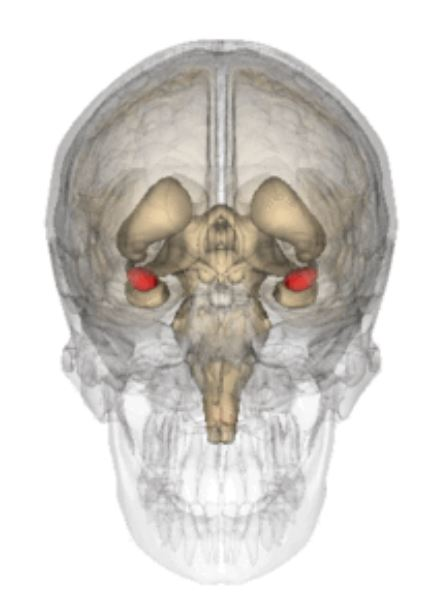
\includegraphics{Figures/2}
\decoRule
\caption[L'amygdale]{Vue 3D de l'amygdale (en rouge).}
\label{fig:amy}
\end{figure}


\subsection{Le cortex orbitofrontal (OF)}

Le cortex orbifrontal [Figure \ref{fig:cortex}, Page \pageref{fig:cortex}] est une région du cortex cérébral qui entre en jeu dans le processus de décision. Il est situé en position antérieure et sur la face inférieure du cortex préfrontal. Il prend son nom des lobes frontaux et du fait qu'il est situé au-dessus des orbites.


Cette partie du cortex préfrontal est en connexion avec le thalamus. Parce qu'il est actif dans les émotions et le système de récompense, le cortex orbitofrontal est souvent considéré comme faisant partie du système limbique.\parencite{cortex}

\begin{figure}[th]
\centering
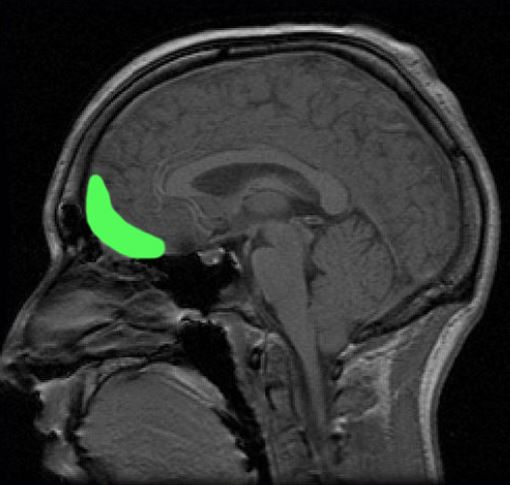
\includegraphics{Figures/3}
\decoRule
\caption[Cortex Orbifrontal]{Emplacement approximatif de cortex orbitofrontal.}
\label{fig:cortex}
\end{figure}


\subsection{Émotions}

Chez les êtres humains, l'émotion inclut fondamentalement « un comportement physiologique, des comportements expressifs et une conscience » \parencite{myers2004theories}

~\par
Les émotions se divisent en plusieurs catégories :

\begin{itemize}
\item Émotions « cognitives » par opposition aux émotions « non cognitives »
\item Émotions instinctives (des amygdales), par opposition aux émotions cognitives (du cortex orbitofrontal)
\item Émotions primaires et secondaires
\end{itemize}

~\par

\begin{figure}[th]
\centering
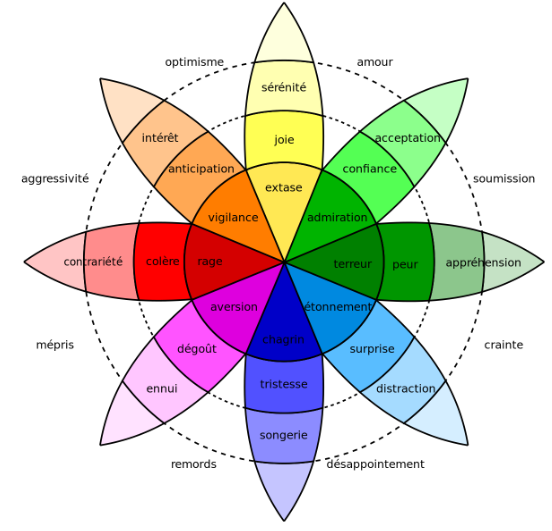
\includegraphics{Figures/emotions.PNG}
\decoRule
\caption[Roue des émotions de Robert Plutchik]{Roue des émotions de Robert Plutchik}
\label{fig:roue}
\end{figure}


\begin{quotation}

 "La théorie psycho-évolutionniste des émotions du professeur et psychologue américain Robert Plutchik \parencite{plutchik} est l'une des méthodes de classification des réactions émotives générales. Plutchik considérait qu'il y avait huit émotions de base [Figure \ref{fig:roue}] : la joie, la peur, le dégoût, la colère, la tristesse, la surprise, la confiance et l'anticipation. Robert Plutchik propose ses 4 émotions fondamentales primaires (la peur, la colère, la joie, la tristesse), qui s'associent à des mécanismes de mémoire et de réflexion pour donner 4 autres émotions fondamentales secondaires (la confiance (liée à la joie), le dégoût (lié à la tristesse), l'anticipation (liée à la colère) et la surprise (liée à la peur)), dont les fonctions respectives seraient la préservation, la protection des acquis, la reproduction, la réintégration, l'incorporation, le rejet, l'orientation et l'exploration. D'autres systèmes de classement des émotions, comme celui de Paul Ekman, ne considèrent que 4 à 6 émotions primaires au lieu de 8, car dans la mesure où les émotions combinées font intervenir des mécanismes de réflexion et de mémoire (par exemple la confiance est liée à un ensemble de souvenirs joyeux) voire de pensée abstraite, il ne s'agit plus d'émotions mais de sentiments par définition.

~\par
Plutchik a organisé ses émotions en paires d'opposés : la joie et la tristesse, la peur et la colère, le dégoût et la confiance, la surprise et l'anticipation. Il faut bien garder à l'esprit que chacune de ces émotions peut varier en intensité, ce qui génère un grand nombre de mots pour les décrire. Par conséquent, il y combine l'idée d'un cercle des émotions et celle d'une palette de couleurs pour représenter cette variation d'intensité et la classer en niveaux, même si la séparation entre les niveaux n'est pas franche. Comme ces dernières, les émotions de base peuvent s'exprimer à divers degrés d'intensité et se combiner l'une à l'autre pour former des émotions différentes. C'est ainsi que Plutchik est venu à définir les dyades primaires [Figure \ref{fig:TbEm}, Page \pageref{fig:TbEm}] (combinaisons de deux émotions de base adjacentes), secondaires (combinaisons d'émotions de base voisines à une émotion près) et tertiaires (combinaisons d'émotions de base voisines à deux émotions près) qui suivent   \parencite{tayari2009modelisation} : "

\end{quotation}


\begin{figure}[th]
\hspace*{-1.9cm} 
\centering
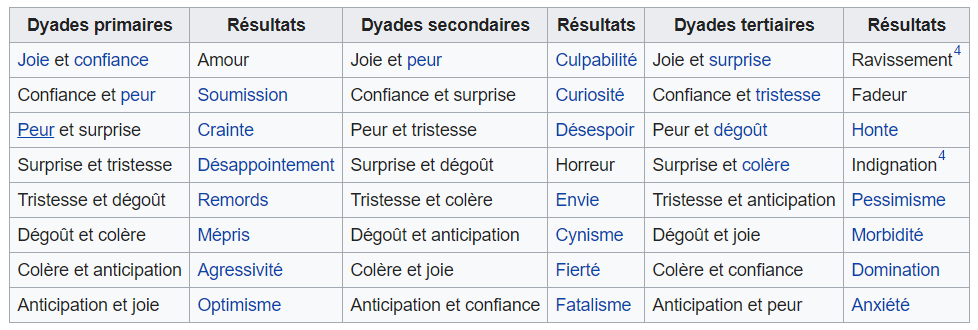
\includegraphics{Figures/tableauEmotions.PNG}
\decoRule
\caption[Tableau de la théorie de Plutchik]{Dyades primaires, dyades secondaires, dyades tertiaires et leurs résultats selon la théorie de Plutchik}
\label{fig:TbEm}
\end{figure}





% Chapter Template

\chapter{État de l'art} % Main chapter title

\label{Chapter2} % Change X to a consecutive number; for referencing this chapter elsewhere, use \ref{ChapterX}

%----------------------------------------------------------------------------------------
%	SECTION 1
%----------------------------------------------------------------------------------------
Dans ce chapitre, nous allons voir les principaux concepts impliqués dans l’implémentation d’agents autonomes; les systèmes multiagents avec quelques exemples d’implémentation; la recherche en “NDM” ou prise de décisions en milieu naturel et quelques modèles issus de ces recherches. Aussi, l’architecture BDI (belief, desire, intention) servant à l’implémentation d’agents autonomes et qui représentent l’un des modèles les plus proches de la cognition humaine, ainsi que d’autres architectures.
Nous verrons aussi comment est abordée l’intelligence artificielle dans les jeux vidéo et de quelle manière elle a évolué depuis l’apparition du jeu vidéo ainsi que deux exemples de jeux célèbres implémentant des IA d’une grande complexité.



\section{SMA (ou Système Multi-agent)}

En informatique, un système multi-agent (SMA) est un système composé d'un ensemble d'agents (un processus, un robot, un être humain, etc.), situés dans un certain environnement et interagissants selon certaines relations. Un agent est une entité caractérisée par le fait qu'elle est autonome, ou du moins partiellement.
Objet de longue date de recherches en intelligence artificielle distribuée, les systèmes multi-agents forment un type intéressant de modélisation de sociétés, et ont à ce titre des champs d'applications larges, allant des sciences humaines, jusqu’aux services militaires et médicaux \parencite{sma}.


%-----------------------------------
%	SUBSECTION 1
%-----------------------------------
\subsection{Exemple de SMA de jeu vidéo}

Les communautés virtuelles que l’on trouve de plus en plus dans les jeux vidéo sont un parfait exemple afin de mieux comprendre le fonctionnement d’un SMA. Par exemple, un jeu qui simulerait la vie d’une famille, plusieurs dimensions composent alors ce SMA.

~\par
Premièrement, un environnement, ayant comme paramètre sa taille et qui pourrait se caractériser par la maison et son jardin. Deuxièmement, les agents de ce SMA disposent d’une quantité d’objets dits “passifs” avec lesquels ils peuvent interagir; ce sera l’équipement de la maison ou encore la nourriture. Ensuite, les agents eux-mêmes, actifs et autonomes, ils sont en contact avec tout ce qui les entoure, leur environnement, les objets qui les composent ou encore les autres agents; on les identifie comme étant “les membres de la famille”. On intègre ensuite le concept d’organisation, constituée des différentes relations entre les objets et les agents, liens familiaux, notions de propriété (qui possède tel ou tel objet). Pour finir, on ajoute des opérateurs qui permettent aux agents d’agir sur leur environnement ou sur les autres agents (le fils peut manger un yaourt, promener son chien ou parler à sa sœur) et de capteurs qui permettent aux agents de connaître les changements d'états de leur environnement et des autres agents (le yaourt est tombé par terre, papa m'a demandé de sortir le chien). Voici donc ce que l'on peut appeler un SMA \parencite{sma}.


\subsection{Exemple de SMA en opération “SWARMM” (Smart Whole Air Mission Model)} \label{ssec:swarm}

Le  programme “SWARMM” \parencite{jones1999automated} a été développé par la division des opérations aériennes de l’organisation australienne de défense, de science et technologies; il a  pour objectif de simuler les opérations des avions de combat pour la flotte aérienne australienne la “Royal Australian Air Force”.

~\par
Chaque pilote est un agent programmé avec dMARS \parencite{dmars1997formal}, un environnement de programmation basé sur le modèle BDI (Belief-desire-intention ou Croyance-désir-intention) et implémenté en FORTRAN et en C. Chacun d'entre eux reçoit des données des modèles physiques équivalentes à celles qu'un pilote reçoit de sa vision et de ses instruments et effectue ce qui suit:

~\par
\begin{itemize}
\item cycle de prise de conscience de la situation lorsque les données sont plus complexes (descripteurs symboliques);
\item  évaluation de la situation, la situation est basée sur les résultats précédents de l'étape précédente;
\item sélection tactique, sélectionnée en fonction de l'ensemble actuel d'objectifs qui a été reconnu lors des étapes précédentes;
\item procédures d'opération: choisies pour mettre en œuvre une tactique.
\end{itemize}

~\par
Plus d'une décennie de contacts étroits, d'entretiens avec des combattants, de briefings de missions et d'implication dans des exercices d'entraînement a été nécessaire afin d’arriver à établir ce cycle. Il s’est avéré être d’une très grande valeur car il permet une intégration simple des procédures standards et de manière très documentée. Il permet aussi aux combattants de décrire facilement leurs connaissances en se basant sur les différentes étapes du cycle. Pour finir, il assure un échange simple compris entre les deux partis, pilotes et programmeurs. Les programmeurs peuvent ainsi décrire leurs résultats et débattre avec les pilotes en utilisant des termes similaires. Ce programme est principalement  basé sur le travail d’équipe et s’est avéré être extrêmement utile pour tester de nouveaux équipements et tactiques.

~\par
L’un des principaux buts du projet était l’introduction d’un pilote (agent humain) dans la boucle de simulation en tant que coéquipier ou adversaire. Il a donc été prouvé que même si pour un observateur extérieur, ce programme ressemble à un vrai pilote, il n’était pas crédible aux yeux des vrais pilotes, et cela aux vues de son comportement extrêmement rationnel et peu naturel \parencite{norling2000enhancing}.


\section{Naturalistic Decision Making (NDM)} \label{ndm}

\begin{quotation}
“L’étude de la NDM  pose la question de comment des individus expérimentés, travaillant individuellement ou en groupes, dans un environnement dynamique, rapide et incertain, identifient et évaluent leurs situations, prennent des décisions et effectuent des actions qui ont des conséquences signifiantes sur eux ainsi que sur l'organisation dans laquelle ils opèrent.” \parencite{zsambok2014naturalistic} \end{quotation} 



Ce terme est apparu en 1989 lors d’ateliers de chercheurs qui avaient pour but d’étudier 
“les prises de décisions dans des contextes réalistes” (médecine, centrales nucléaires, planification exécutive). Leurs études ont montrés que les théories classiques sur les prises de décisions n’étaient tout simplement pas applicables dans le monde réel. Ils ont aussi prouvé que même lorsque les agents étaient entraînés à faire des choix rationnels, ces derniers ne le faisaient que rarement.

~\par
Il en a ainsi émergé une meilleure compréhension sur la manière dont nous procédons pour prendre des décisions dans des situations complexes. Dans certains cas, nous procédons effectivement de manière rationnelle, où, une multitude d’options sont générées et la “meilleure” est sélectionnée, mais il existe d’autres stratégies qui sont plus communément utilisées.

~\par
La recherche dans ce domaine est principalement destinée à la conception d’aides à la décision, mais ces résultats peuvent également être utilisés pour développer de meilleurs modèles cognitifs pour les humains lors des simulations.

~\par
Orasanu et Connolly \parencite{orasanu1993reinvention} énumèrent huit facteurs qui caractérisent les paramètres de prise de décisions en milieu naturel. De nombreuses études de prise de décisions classiques ignorent ou limitent délibérément ces facteurs, ce qui rend la théorie du choix rationnel plus facile à appliquer.

~\par

Ces facteurs sont:
\begin{itemize}
\item problèmes mal structurés;
\item environnements dynamiques incertains;
\item objectifs changeants, mal définis ou concurrents;
\item boucles d'actions / de rétroactions;
\item le stress dû au temps;
\item des enjeux trop élevés;
\item plusieurs joueurs;
\item objectifs organisationnels et normes.
\end{itemize}

~\par
Tous ces facteurs ne sont pas présents dans un contexte dit “naturel”, mais chacun ajoute une complexité au problème.


\subsection{Modèles de NDM}

Plusieurs modèles de prise de décisions en milieu naturel ont été proposés, mais à ce jour,
aucun d’entre eux ne rend compte du spectre complet des décisions pouvant être prises dans un contexte naturel. Lipshitz \parencite{lipshitz1993converging} donne un résumé de neuf modèles qu’il souligne être non contradictoires, mais illustrent les différents types de prise de décision qui peuvent être utilisés.

~\par
Notez que les chercheurs en NDM s'intéressent généralement aux personnes qui sont expérimentées dans leurs domaines. Hubert Dreyfus explique le modèle d’acquisition de compétences en cinq étapes dans \parencite{dreyfus2014intuitive}, avec des niveaux allant de novice (quelqu'un qui débute dans  le domaine, comme un apprenti pilote), à un expert (quelqu'un qui est très habile dans son activité). La plupart des modèles NDM supposent un certain niveau d'expertise dans le domaine, pas nécessairement expert, mais certainement pas novice. L’un des modèles les plus connus est celui de Klein intitulé  “recognition-primed decision making”, modèle (RPD), ou “la prise de décision axée sur la reconnaissance” \parencite{klein2017sources}, illustré à la figure \ref{fig:klein}.

~\par 
Comme le souligne Klein lui-même «Le modèle RPD n'est pas issu de recherches en NDM» (\parencite{klein2017sources}, p.102), mais des études d’experts dans divers domaines montrent qu’une grande partie de leurs décisions sont prises de cette façon (figure \ref{fig:klein}). La chose importante à noter à propos de ce modèle est l'accent qui est mis sur l'évaluation de la situation. Une fois que le décideur a reconnu la situation, il existe quatre sous-produits:

\begin{enumerate}

\item il / elle s'attend à ce que certaines choses se produisent mais pas d'autres;
\item il / elle fait attention à certains signaux pour soutenir le diagnostic;
\item il existe une certaine compréhension des objectifs qu'il est plausible de réaliser;
\item certaines actions sont susceptibles de réussir.
\end{enumerate}

Le décideur choisit ensuite une action, exécute une rapide simulation mentale de
celle-ci, et s'il/elle pense que cela va réussir, la met en œuvre. Une fois que le plan d’action  a été sélectionné et qu’il est entamé, la situation est surveillée pour s’assurer qu’elle se déroule comme prévu, sinon, d’autres actions pourraient être envisagées, mis à part cette éventualité, le décideur n'envisage pas d'autres options. Dans le modèle RPD, un opérateur expérimenté
choisira généralement «automatiquement» un plan d’action une fois que la situation est
reconnue, et que ce plan d’action est susceptible d’être celui qui a donné  auparavant
des résultats positifs dans la même situation.


\begin{figure}[th]
\centering
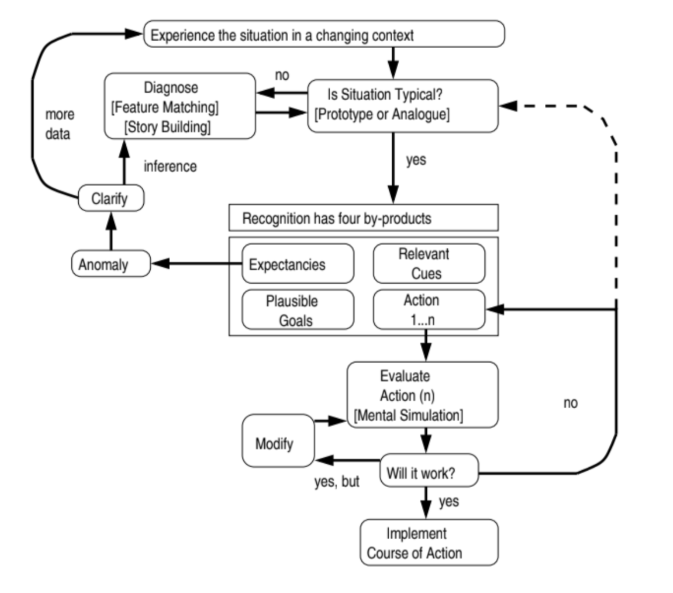
\includegraphics{Figures/klein.PNG}
\decoRule
\caption[ La version intégrée  du modèle de Klein de décision axée sur la reconnaissance] { La version intégrée  du modèle de Klein de décision axée sur la reconnaissance
(Figure 7.1 du livre “Sources of Power” by G. Klein 1998 \parencite{klein2017sources}) }
\label{fig:klein}
\end{figure}


~\par
Le modèle de la figure \ref{fig:klein} exprime l’idée qu’une personne qui acquiert de l’expertise est plus susceptible 
de reconnaître les subtilités entre les situations et de choisir un plan d’action en conséquence.



~\par

\section{Une brève histoire des jeux dans la recherche sur l'IA}

Les jeux ont une longue histoire dans la recherche sur l'IA, remontant au moins à 1949 lorsque Claude Shannon (peu après avoir développé l'entropie d'informations) s'est intéressé à l'écriture d'un programme informatique pour jouer au jeu d'échecs \parencite{unity2}. Dans son article «Programmer un ordinateur pour jouer aux échecs», Shannon écrit:

~\par
“La machine à échecs est un système idéal pour commencer, car: 

~\par
\begin{enumerate}
\item le problème est clairement défini à la fois dans les opérations autorisées (les mouvements) et dans le but ultime (le mat); 
\item il n'est ni si simple jusqu'à être trivial ni trop difficile; 
\item les échecs sont généralement considérés comme nécessitant une «réflexion»; une solution à ce problème nous obligera soit à admettre la possibilité d'une pensée mécanisée, soit à restreindre davantage notre concept de «pensée»; 
\item la structure discrète des échecs s’intègre parfaitement dans la nature numérique des ordinateurs modernes.”

\end{enumerate}

C'était en 1949.

~\par
Depuis lors, il existe un intérêt considérable pour la création de programmes informatiques capables de jouer à des jeux de manière aussi habiles que des joueurs humains, parfois même en battant les meilleurs. Shannon a inspiré le travail fondateur d’Arthur Samuel sur Checkers entre les années 1950 et 1960. Si le programme de Samuel n’a pas pu battre les experts, il a été considéré comme une réalisation majeure, car il s’agissait du premier programme à utiliser efficacement les procédures de recherches heuristiques et les méthodes basées sur l’apprentissage \parencite{unity1}.


~\par
Chinook, un programme de contrôleurs mis au point à l’Université d'Alberta en 1989, a commencé à battre les joueurs humains, et dès 1994, les meilleurs joueurs pouvaient au mieux être à égalité avec la machine. Cette tendance s’est poursuivie avec d’autres jeux de plateau à 2 joueurs tels que le backgammon (avec TD-Gammon de Gerald Tesauro, 1992-2002) et le jeu d'échecs (lorsque Deep Blue d’IBM a battu Garry Kasparov, 1997), et plus récemment avec Go.

~\par
Une avancée scientifique importante de ces dernières années a été celle où, en 2016, AlphaGo de DeepMind a battu le champion du monde Lee Sedol 18 fois 4 à 1, faisant l’objet du documentaire Netflix, AlphaGo \parencite{unity2}. 



\section{BDI ( Belief-Desire-Intention)}

Les agents du modèle BDI sont basés sur les concepts philosophiques d'intentions, de plans et de raisonnements pratiques développés par Bratman \parencite{bratman1987intention}. Ce modèle est basé sur la psychologie populaire, c'est-à-dire la manière dont nous pensons. Le modèle fournit une première approximation de la cognition humaine, mais il reste encore beaucoup à faire pour l’affiner.


\subsection{Belief}

Les croyances d'un agent sont sa vision du monde, qui n'est pas nécessairement la même chose que l'état du monde, car les capteurs peuvent être imparfaits, en effet, les informations fournies peuvent être à la fois incomplètes et bruyantes.

\subsection{Desire}

Plutôt que les désirs d’un agent, nous nous référons à ses objectifs. Ceux-ci donnent l'état du monde dans lequel l'agent souhaite être et doit être cohérent.


\subsection{Intention}

Ses intentions sont les plans qu'il exécute actuellement. Il peut y avoir plus d'un plan en cours, car un agent peut travailler simultanément à plusieurs objectifs (non conflictuels). Une fois qu'un agent a formulé une intention (c.-à-d. il sélectionne un plan), il est en quelque sorte engagé dans ce plan - il continue de l'exécuter (ou du moins a l'intention de l'exécuter) jusqu'à ce que l'objectif soit atteint ou qu’il devienne impossible à atteindre en suivant ce même plan, l'objectif devient alors inutile. 
Un plan est une «recette» pour atteindre un objectif particulier. C'est une séquence d'actions et/ou de sous-objectifs à réaliser. Si une étape de la séquence échoue, le plan lui-même échouera. L'une des caractéristiques d'un système BDI est que, lorsqu'un plan échoue, l'agent réessaye (si possible). Il tentera de trouver un autre moyen d’atteindre l’objectif en tenant compte du fait que le monde (et donc les convictions de l’agent ou son désir) est en train de changer. Un agent stocke ses plans dans une bibliothèque de plans.


\subsection{Agent BDI} \label{bdiA}

L'agent montré à la figure \ref{fig:bdi}, page \pageref{fig:bdi} \parencite{norling2000enhancing} passe par un cycle continu de:

\begin{enumerate}
\item visualiser son environnement;
\item raisonner sur les croyances, les objectifs et les intentions;
\item accomplir une ou plusieurs actions.
\end{enumerate}

Ce cycle est très similaire à celui utilisé dans SWARMM section \ref{ssec:swarm}, qui sépare la deuxième étape en deux étapes: évaluation de la situation suivie de la sélection tactique. En effet, SWARMM est implémenté en utilisant une architecture BDI. Au cours de la phase de raisonnement du cycle, l'agent doit raisonner sur les croyances (si et comment elles devraient changer), les objectifs (les changements de croyances peuvent affecter la faisabilité des objectifs) et les intentions (les changements d'objectifs peuvent amener l'agent à abandonner certaines intentions et / ou d’en créer de nouvelles). L'agent doit également décider quelle action (ou quelles actions) effectuer ensuite, à partir des intentions actuelles.


\begin{figure}[th]
\centering
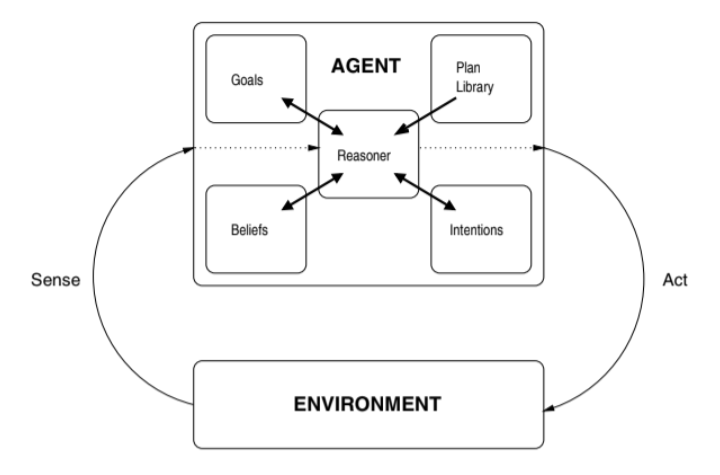
\includegraphics{Figures/bdi.PNG}
\decoRule
\caption[ Structure d’un agent BDI ] { Structure d’un agent BDI }
\label{fig:bdi}
\end{figure}


~\par
Lorsqu'il existe plusieurs plans disponibles pour atteindre un objectif donné, l'agent utilise en théorie un choix rationnel pour sélectionner un plan \parencite{bratman1988plans}. C'est-à-dire que les avantages de tous les plans applicables sont évalués et que le «meilleur» est sélectionné. Cependant la recherche en NDM indique que ce n'est pas ainsi que les agents humains prennent leurs décisions, et c'est sur cela que le travail doit être fait pour  améliorer le modèle BDI .

~\par
Dans les implémentations pratiques d'architectures BDI, telles que JACK \parencite{jack} ou dMARS \parencite{dmars1997formal}, chaque plan est conçu pour gérer un objectif particulier dans un contexte particulier. Dans ces systèmes, le "contexte" est un ensemble de conditions que l'agent doit croire vraies. Cela permet au programmeur de spécifier différentes manières d'atteindre le même objectif dans différentes situations, mais il est également possible d'avoir plusieurs plans applicables dans une situation donnée (lorsque les contextes se chevauchent).







\section{Autres modèles et architectures}

\subsection{CogAff} \label{cogaff}

CogAff est un modèle de traitement de l'information proposé par Sloman \parencite{sloman2005architectural}. Il comprend trois niveaux, à savoir: réactif, délibératif et réflexif (méta-gestion). 
Chaque niveau comprend des mécanismes de perception, des mécanismes de traitement centralisés et des mécanismes d'action. L'architecture possède un mécanisme d'alarme ainsi que des communications d'informations entre toutes les parties de l'architecture. Le mécanisme d'alarme fonctionne de manière centralisée et s'apparente au mécanisme d'interruption.

~\par

H-CogAff est un exemple particulier de CogAff expliquant les phénomènes mentaux humains. Chaque niveau supporte différentes catégories d'émotions. «D'autres subdivisions sont nécessaires pour couvrir toute la variété des émotions humaines, d'autant plus que les émotions peuvent changer de caractère au fil du temps, à mesure qu'elles grandissent» \parencite{sloman2005architectural}.


\subsection{CLARION}

CLARION a une structure similaire aux trois niveaux de traitement de l’information (section \ref{cogaff}). C'est une architecture cognitive qui comporte deux niveaux: le niveau implicite (similaire aux niveaux réactifs et de routines) et le niveau explicite (similaire au niveau réflexif). Le niveau implicite est le niveau inférieur et code les connaissances implicites. Il utilise un réseau de neurones multi-couches avec Q-learning \parencite{watkins1992q} pour acquérir des connaissances implicites. Le niveau explicite est le niveau supérieur et code la connaissance explicite. Il utilise un apprentissage ponctuel pour acquérir des connaissances explicites.

~\par
Le niveau le plus bas et le niveau le plus élevé échangent leurs apprentissages au moyen d'un apprentissage ascendant et descendant. Chaque niveau comprend quatre sous-systèmes fonctionnels distincts:

\begin{enumerate}
\item un sous-système centré sur l'action pour contrôler les actions;
\item un sous-système non centré sur l'action pour conserver les connaissances générales implicites ou explicites;
\item un sous-système méta-cognitif pour surveiller, diriger et modifier les opérations de tous les sous-systèmes;
\item un sous-système de motivation pour fournir les motivations sous-jacentes de la perception, de l'action et de la cognition, en termes d'impulsion et de rétroaction.
\end{enumerate}

\subsection{SHAME}

SHAME (Architecture évolutive et hybride pour le mimétisme des émotions) est un modèle émotionnel ou système simulant l'état émotionnel d'un agent agissant dans un environnement virtuel présenté par Kesteren en 2001 \parencite{kesteren2001supervised}. Il a construit un modèle de simulation à base d'agents appelés «GridWorld». SHAME implémente la fonction d’affect similaire à la fonction d’affect dans le niveau de réflexion et des fonctions de motivation et de comportement similaires à celles du niveau réactif. Il utilise un réseau de neurones pour apprendre comment l'état émotionnel devrait être influencé par la survenue de stimuli.


\subsection{Zamin}

Zamin est un environnement de simulation de vie artificielle pour évaluer les capacités des agents à produire un comportement émotionnel et à prendre de meilleures décisions, développé par Zadeh, Shouraki et Halavati \parencite{zadeh2006emotional}. Ces derniers ont mis en place cet environnement afin d’étudier le possible rôle des émotions dans la gestion des ressources mentales. Ils utilisent uniquement un comportement positif/négatif et un comportement d'approche/d'évitement (uniquement la fonctionnalité du niveau réactif) dans un environnement de type prédateur-proie.


\section{L'évolution de l’IA dans les jeux vidéo}

L’IA n’a pas tant évolué que ça au fil des années, elle fonctionne toujours sur les deux principes de \parencite{youtubeIA}:

~\par
\begin{itemize}

\item  pathfinding: aller d’un point A à un point B, déjà utilisé il y a 20 ans et encore utilisé;

\item  state machine: un agent autonome peut être dans les différents états et changer de l’un à l’autre.

\end{itemize}

~\par
L’IA a  évolué depuis dans tous les domaines, grâce à un concept clé qui est le deep learning, le fait d'alimenter un agent autonome avec des millions de données issues d'expériences diverses. 

~\par
Mais les constructeurs de jeux vidéo ne peuvent pas se reposer sur cette technologie, car les agents autonomes basés sur du deep learning ne sont pas prédictibles, et cela pose un grand problème à ces mêmes constructeurs car ils ne peuvent pas prévoir des scénarios précis en utilisant ce type d’IA, c’est pourquoi ils se basent plutôt sur IA ayant des paramètres, qui simulent des comportements aléatoires, mais n’en sont pas vraiment. Simulent, car celles-ci ont des comportements prédéfinis et paramétrés, mais changeants au changement dans leur environnement mais toujours prédictibles, ceux-ci sont toujours basées sur les deux principes fondamentaux cités plus haut.

~\par
Une IA qui réagit aux émotions du joueur et construit des plans d’action selon ceux-ci peut sembler improbable, mais la recherche dans ce domaine avance rapidement.

~\par
En effet grâce à une technique appelée “génération procédurale” \parencite{generation}, popularisée grâce au jeu “No man’s sky”, cette IA permettait la création d’univers spatiaux totalement aléatoire mais cohérents.

~\par
Les recherches à partir de cette technique visent à réaliser des jeux entiers en “génération procédurale”, l’univers, les personnages, leurs attitudes vis-à-vis du joueur etc.

~\par
Les développeurs de jeux vidéo pourront donc créer, non seulement des univers procéduraux et aléatoires, mais aussi construire une expérience de jeu propre aux goûts de chaque joueur, qui s’améliorera au fil du temps que le joueur passe sur le jeu, ce qui lui permettra de s’alimenter de ses goûts et préférences et de les implémenter en temps réel \parencite{youtubeIA}.

~\par
Les jeux cités dans les sections \ref{red} et \ref{sims0} sont parmi les meilleurs dans l’implémentation d’agents autonomes (personnages non jouables) dans l’industrie du jeu vidéo. C’est aussi, en partie, ce qui fait leur grand succès auprès des joueurs, le fait que tout rappelle le monde réel.


%\section{Analyse de jeux existants bénéficiant d’une IA complexe}

\subsection{Red Dead Redemption 2}\label{red}

Dans ce jeu doté d’immenses paysages sorti tout droit d’un western, le joueur peut parler à n’importe quel personnage en appuyant sur le déclencheur gauche et en sélectionnant une interaction positive ou négative. Celles-ci en pour conséquence des actions différentes à chaque fois, en fonction du contexte: les vêtements du joueur, les taches de sang, la boue, l’emplacement, ce que fait l’agent autonome au moment de la prise de contact, la côte d’honneur, la quantité d’alcool que le joueur a consommé, et plus encore \parencite{red}.


~\par
Comme on peut le voir ici, les actions des agents ne sont pas complètement aléatoires, elles sont programmées, mais ce qui fait leur force et donne l’illusion du “monde réel ”, c’est le nombre épatant de paramètres entrants en compte pour déterminer quelle action va entreprendre l’agent, un petit détail qui change dans leur environnement peut engendrer une modification dans le déroulement d’une situation (un cheval qui passe à une grande vitesse, un autre agent qui dit un gros mot etc.). 

~\par
Les émotions que possède chaque personnage non jouable ne sont pas nourries par une grande quantité de données comme on peut le trouver dans d’autres secteurs utilisant l’intelligence artificielle,  mais par une quantité de conditions qui déterminent les différents états émotionnels, ce qui rend les agents prédictibles et permet aux constructeurs de construire une histoire cohérente, avec une dose de mystère maîtrisée.

~\par
En plus de l’implémentation d’une IA complexe, une énorme quantité de gestes et d’animations subtiles l’accompagnent, ce qui élève le jeu entier à un niveau beaucoup plus réaliste.

~\par
Par exemple le fait que tous les dialogues se passent en temps réel dans le jeu plutôt que dans une liste d'options de dialogue sur un écran statique. C’est une nouvelle approche de l’interaction dans le jeu - déclenchée de la même manière que vous tirez avec une arme à feu sur un agent autonome - et vous donne l’illusion que tout est possible. Plutôt que d'interagir avec ce monde en tuant et en mutilant, Red Dead Redemption 2 donne des mots aussi puissants que des balles. 

~\par
Ou encore,  "si un témoin vous surprend en train de faire quelque chose, Arthur (le personnage joué par l’utilisateur) dit: " Ah, merde ... " car vous devez les pourchasser", ajoute David Hynd, programmeur en charge de l'IA. “Ou bien, si vous pénétrez dans un salon, l'IA peut s'arrêter dans sa tâche et la musique peut cesser de jouer - l'IA vous regardera un instant avant de revenir sur ses affaires. Ou pas, s'ils vous voient comme une menace. Et c’est incroyable de voir comment Arthur peut chanter et fredonner, ou comment on peut  transformer le cours des choses en interagissant avec les agents autonomes quand il se saoule”.

~\par
Je pense que ce sont les petits détails qui font que tout paraît si réaliste.




\subsection{The Sims 4}\label{sims4}

Le 2 septembre 2014, le studio Maxis d'Electronic Arts lancera The Sims 4. Comme toute suite, le jeu ressemblera à son vieil ami: on peut toujours créer nos propres “sims”, construire notre propre maison, déterminer notre propre vie et, espérons-le, ne pas tuer ni négliger notre propre avatar. Mais la technologie sous-jacente - les os et les nerfs qui maintiennent l’univers ensemble - fait actuellement l’objet d’une mise à niveau majeure pour la quatrième génération \parencite{simsArticle}.

~\par
L’une des avancées à consister à peaufiner le système de routage, ou la façon dont les sims naviguent. Après avoir étudié le comportement social humain, les développeurs ont rendu les sims moins gênants et plus crédibles. “Les sims peuvent maintenant franchir les portes sans rester coincés, mais il est extrêmement difficile d'y arriver" dit Pearson Ingebretson - Ingénieur logiciel pour the Sims 4. 

~\par
Au cœur de chaque jeu des sims se trouve son intelligence artificielle, son réseau infini de modèles (figure \ref{fig:sims}) et ses résultats possibles qui font tourner le monde en coulisses. Dans les jeux, l'intelligence artificielle fait généralement référence à la manière dont l'environnement, et en particulier les personnages non joueurs, interagissent avec le monde et le joueur. Cependant, la franchise Les Sims se distingue.

\begin{figure}[th]
\centering
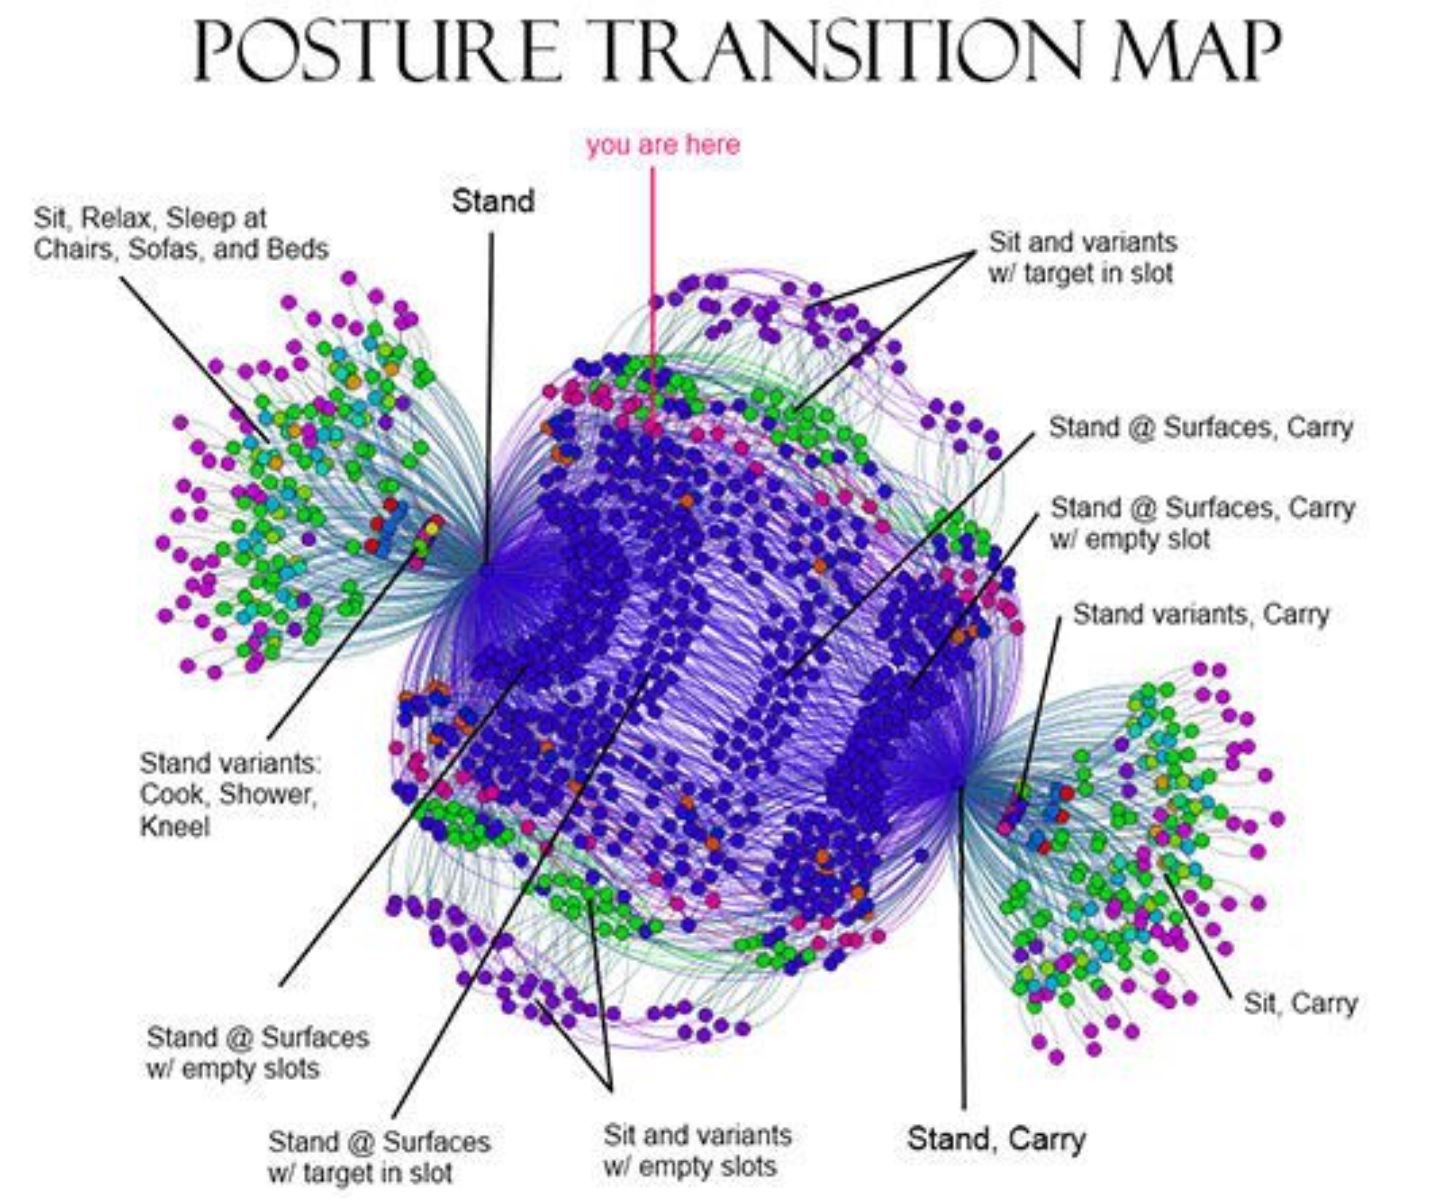
\includegraphics{Figures/sims.JPG}
\decoRule
\caption[Le potentiel des conséquences d'un changement de posture d'un Sim dans Les Sims 4]{Cette image visualise le potentiel des conséquences d'un changement de posture d'un Sim dans Les Sims 4}
\label{fig:sims}
\end{figure}


~\par
"Dans de nombreux autres jeux, l'IA est étrangère au joueur quant à la manière dont elle se comporte. L'IA commande aux personnages de faire des choses fondamentalement différentes de celles des joueurs ... Ils opèrent dans un monde différent avec des possibilités différentes", explique Ingebretson. “Dans Les Sims, si vous restez assis à regarder votre ordinateur pendant un moment, l'IA prendra le contrôle et contrôlera également les actions de vos sims. Cela signifie que notre IA  doit prendre des décisions plus crédibles afin que le cours de l’action reste cohérent “\parencite{simsArticle}.

~\par
Écouter Ingebretson qui décrit les tenants et les aboutissants de l’intelligence artificielle dans The Sims 4 ressemble à un cours de psychologie humaine. À la base, l'IA travaille avec l'interaction de deux mécanismes: les commodités et les courbes d'utilité. Les commodités représentent l'état interne d'un Sim, tandis qu'une courbe d'utilité dicte le désir d’un avatar à améliorer ses commodités. Chaque interaction ouvre une série d'améliorations possibles. "Par exemple, si un Sim boit une tasse de café, son énergie va monter mais sa vessie va baisser", dit Ingebretson. Comme dans le monde réel, tout est un compromis. Ainsi, lorsqu'il prend chaque décision, un Sim considère toutes les actions possibles, analyse leurs résultats, référence la courbe d'utilité et sélectionne la meilleure. Cependant, ces actions sont quelque peu aléatoires de par leur conception, de sorte que l'IA puisser donner l’illusion qu’elle est imprévisible.

~\par
Cet échange en une fraction de seconde entre la prise de contrôle de l’IA et du joueur est ce que Ingebretson appelle «autonomie», ou lorsqu'un sim est en pilote automatique. Dans les jeux précédents des Sims, l’autonomie était un système de départ et d’arrêt. Une fois qu'un sim a terminé avec une action, il s'exécute de manière autonome. Dans Les Sims 4, les développeurs ont amélioré l'efficacité de l'IA en créant une hiérarchie d'autonomie. "Au lieu de tout considérer dans le monde entier chaque fois qu'un Sim décide quoi faire, nous évaluons d'abord tous les produits de base et déterminons quels types d’actions sont les plus importantes pour le Sim", explique Ingebretson. "Cela nous permet d'éliminer de nombreuses possibilités." Cela signifie que les Sims deviennent plus rapides et plus efficaces pour prendre des décisions et peuvent effectuer plusieurs tâches plutôt que de suivre un script strict «d'abord ceci, ensuite cela» \parencite{simsArticle}.

~\par
Toutes ces améliorations et ces avancées rendent un jeu plus naturel, mais quand est-ce qu’un système d'intelligence artificielle devient-il trop efficace? "C'est un sujet intéressant que nous traitons dans chacun de ces projets, car nous pouvons continuer à rendre les Sims suffisamment intelligents pour mener leur propre vie", a déclaré Pearson. "Qu'est-ce qui est trop intelligent?"

~\par

Laissée à ses propres appareils parfaitement optimisés, l'IA pourrait facilement prendre le contrôle et jouer au jeu pour vous, laissant ainsi aux Sims effectuer un nombre anormal d'actions en même temps ou annuler l'interaction du joueur. L’équipe a introduit des seuils de retard et d’attention pour limiter artificiellement le système. "Il est impossible pour un cerveau humain de gérer autant de flux d'entrées", explique Ingebretson. "Pour les Sims, nous construisons un modèle de la vie humaine. Nous devons modéliser les fautes des gens ainsi que leur efficacité" \parencite{simsArticle}. 

~\par
Nous pouvons apercevoir que l'approche dans Les Sims 4 afin de rendre l’IA plus crédible est différente du cas précédent, même si les deux approches ont des similitudes dans la complexité de leur modèle, qui consiste à alimenter les personnages d’un grand nombre de conditions détaillées et en cascade ( un geste, une quantité d’alcool consommée, une intonation...), avec des scénarios différents pour chaque état, c’est tout ces détails qui donnent l’illusion de la réalité.

~\par
En plus de cela, Les Sims 4 propose un système tout à fait novateur, qui consiste en la prise de contrôle de l’IA du personnage joué par l’utilisateur lors des moments où celui-ci est au repos (quand le joueur laisse tourner le jeu sans y toucher). Mais celle-ci ne le fait pas n’importe comment, elle le fait tout en restant cohérente avec l’état précédent de l’agent, par exemple si le personnage est en train de boire de l’eau et que l’IA intervient et en prend le contrôle, elle le pousse à laver son verre, avant de l'essuyer de le ranger dans l’évier.

~\par
En plus de cela, les fautes des gens ainsi que leurs moments d'inattention et de faiblesse ont aussi été modélisés, non pas de manière directe, mais en introduisant des seuils de retards dans la succession des actions, afin que celles-ci aient l’air naturelles, et qu’elles ne ressemblent pas à un flot ininterrompu d’actions, comportement  qui n’est pas compréhensible par l’homme.
 
% Chapter Template

\chapter{Background} % Main chapter title

\label{Chapter3} % Change X to a consecutive number; for referencing this chapter elsewhere, use \ref{ChapterX}

%----------------------------------------------------------------------------------------
%	SECTION 1
%----------------------------------------------------------------------------------------

\section{SMA (ou Système Multi-agent)}

En informatique, un système multi-agent (SMA) est un système composé d'un ensemble d'agents (un processus, un robot, un être humain, etc.), situés dans un certain environnement et interagissant selon certaines relations. Un agent est une entité caractérisée par le fait qu'elle est, au moins partiellement, autonome.
Objet de longue date de recherches en intelligence artificielle distribuée, les systèmes multi-agents forment un type intéressant de modélisation de sociétés, et ont à ce titre des champs d'applications larges, allant des sciences humaines, jusqu’aux services militaires et médicaux. \parencite{sma}


%-----------------------------------
%	SUBSECTION 1
%-----------------------------------
\subsection{Exemple de SMA de jeu vidéo}

Les communautés virtuelles que l’on trouve de plus en plus dans les jeux vidéo sont un parfait exemple afin de mieux comprendre le fonctionnement d’un SMA, par exemple, un jeu qui simulerait la vie d’une famille, plusieurs dimensions composent alors ce SMA.

~\par
Premièrement, un environnement ayant comme paramètre sa taille qui pourrait se caractériser par la maison et son jardin. Deuxièmement, les agents de ce SMA disposent d’une quantité d’objets dits “passifs” avec lesquels ils peuvent interagir, ce sera l’équipement de la maison ou encore la nourriture. Ensuite, les agents eux-mêmes, actifs et autonomes, ils sont en contact avec tout ce qui les entoure, leurs environnements, les objets qui le composent ou encore les autres agents, on les identifie comme étant “les membres de la famille”. On intègre ensuite le concept d’organisation, constitué des différentes relations entre les objets et les agents, liens familiaux, notions de propriété(qui possède tel ou tel objet). Pour finir, on ajoute des opérateurs qui permettent aux agents d’agir sur leur environnement ou sur les autres agents (le fils peut manger un yaourt, promener son chien ou parler à sa sœur)
Enfin, on intègre un ensemble d'opérateurs qui permettent aux agents d'agir sur les objets ou sur les autres agents (le fils peut promener son chien ou manger un yaourt ou parler à son père), et de capteurs qui permettent aux agents de connaître les changements de l'environnement et des autres agents (le yaourt est tombé par terre, papa m'a demandé de sortir le chien). Voici donc ce que l'on peut appeler un SMA. \parencite{sma}


\subsection{Exemple de SMA en opération “SWARMM” (Smart Whole Air Mission Model)} \label{ssec:swarm}

le  programme “SWARMM” a été développé par la division des opérations aériennes de l’organisation australienne de défense de science et technologies, il a  pour objectif de simuler les opérations des avions de combat pour la flotte aérienne australienne “La Royal Australian Air Force”.

~\par
Chaque pilote est un agent programmé avec dMARS, un environnement de programmation basé sur BDI(Belief-desire-intention ou Croyance-désir-intention) implémenté en FORTRAN et en C, chacun d'entre eux recevant des données des modèles physiques équivalents à ceux qu'un pilote reçoit de sa vision et de ses instruments et effectuant ce qui suit:

~\par
\begin{itemize}
\item Cycle de prise de conscience de la situation lorsque les données sont plus complexes (descripteurs symboliques)
\item  Évaluation de la situation, la situation est basée sur les résultats précédents de l'étape précédente.
\item Sélection tactique, sélectionnée en fonction de l'ensemble actuel d'objectifs qui a été reconnu lors des étapes précédentes
\item Procédures d'opération: choisies pour mettre en œuvre une tactique.
\end{itemize}

~\par
Plus d'une décennie de contacts étroits, d'entretiens avec des combattants, de briefing de missions et d'implication dans des exercices d'entraînement a été nécessaire afin d’arriver à établir ce cycle, il s’est avéré être d’une très grande valeur car il permet une intégration simple des procédures standard et de manière très documentée, il permet aussi aux combattants de décrire facilement leurs connaissances en se basant sur les différentes étapes du cycle et pour finir, il assure un échange simple compris entre les deux partis, pilotes et programmeurs, les programmeurs peuvent ainsi décrire leur résultat et débattre avec les pilotes en utilisant des termes similaires, il est principalement  basé sur le travail d’équipe et s’est avéré être extrêmement utile pour tester de nouveaux équipements et tactiques.

~\par
L’un des principaux buts du projet était  l’introduction d’un pilote (agent humain) dans la boucle de simulation en tant que coéquipier ou adversaire, il a donc été prouvé que même si pour un observateur extérieur ce programme ressemble à un vrai pilote, il n’était pas crédible aux yeux des vrais pilotes, et cela aux vues de son comportement extrêmement rationnel et peu naturel. \parencite{norling2000enhancing}


\section{NDM ( Naturalistic Decision Making)}

\begin{quotation}
“ L’étude de la NDM  pose la question de comment des individus expérimentés, travaillant individuellement ou en groupes, dans un environnement dynamique, rapide et incertain, identifient et évaluent leurs situations, prennent des décisions et effectuent des actions qui ont des conséquences signifiantes sur eux ainsi que sur l'organisation dans laquelle ils opèrent ” \parencite{zsambok2014naturalistic} \end{quotation} 



Ce terme est apparu en 1989 lors d’ateliers de chercheurs qui avaient pour but d’étudier 
“les prises de décisions dans des contextes réalistes” (médecine, centrales nucléaires, planification exécutive), leurs études ont montrés que les théories classiques sur les prises de décisions n’étaient tout simplement pas applicables dans le monde réel, ils ont aussi prouvé que même lorsque les agents étaient entraînés à faire des choix rationnels, ces derniers ne le faisaient que rarement.

~\par
Il en a ainsi émergé une meilleure compréhension sur la manière dont nous procédons pour prendre des décisions dans des situations complexes, dans certains cas, nous procédons effectivement de manière rationnelle, où, une multitude d’options sont générées, et la “meilleure” est sélectionnée, mais il existe d’autres stratégies qui sont plus communément utilisées.

~\par
La recherche dans ce domaine est principalement destinée à la conception d’aides à la décision, mais ces résultats peuvent également être utilisés pour développer de meilleurs modèles cognitifs pour les humains lors des simulations.

~\par
Orasanu et Connolly \parencite{orasanu1993reinvention} énumèrent huit facteurs qui caractérisent les paramètres de prises de décisions en milieu naturel. De nombreuses études de prise de décision classiques ignorent ou limitent délibérément ces facteurs, ce qui rend la théorie du choix rationnel plus facile à appliquer.

~\par

Ces facteurs sont:
\begin{itemize}
\item Problèmes mal structurés.
\item Environnements dynamiques incertains.
\item Objectifs changeants, mal définis ou concurrents.
\item Boucles d'action / de rétroaction.
\item Le stress dû au temps.
\item Des enjeux trop élevés.
\item Plusieurs joueurs.
\item Objectifs organisationnels et normes.
\end{itemize}

~\par
Tous les facteurs ne sont pas présents dans un contexte dit “naturel”, mais chacun ajoute une complexité au problème.


\subsection{Modèles de NDM}

Plusieurs modèles de prise de décision naturaliste ont été proposés, mais à ce jour,
aucun d’entre eux ne rend compte du spectre complet des décisions pouvant être prises dans un contexte naturel. Lipshitz \parencite{lipshitz1993converging} donne un résumé de neuf modèles qu’il souligne entre non contradictoires, mais illustrent les différents types de prise de décision qui peuvent être utilisés.

~\par
Notez que les chercheurs dans ce domaine s'intéressent généralement aux personnes qui sont expérimentées dans leur domaine. Hubert Dreyfus explique «le modèle d’acquisition de compétences en cinq étapes dans \parencite{dreyfus2014intuitive}, avec des niveaux allant de novice (quelqu'un qui débute dans  le domaine, comme un apprenti pilote), à un expert (quelqu'un qui est très habile et immergé dans son activité). La plupart des modèles NDM supposent un certain niveau d'expertise dans le domaine, pas nécessairement expert, mais certainement pas novice. L’un des modèles les plus connus est celui de Klein intitulé  “recognition-primed decision making” Modèle (RPD),  ou “la prise de décision axée sur la reconnaissance”. \parencite{klein2017sources}, illustré à la Figure \ref{fig:klein}.

~\par
Comme le souligne Klein lui-même «Le modèle RPD n'est pas issue de recherches en NDM »(\parencite{klein2017sources}, p.102), mais des études d’experts dans divers domaines montrent qu’une grande partie de leurs décisions sont prises de cette façon (voir le tableau 7.2 dans \parencite{klein2017sources}). La chose importante à noter à propos de ce modèle est l'accent qui est mis sur l'évaluation de la situation. Une fois que le décideur a reconnu la situation, il existe quatre sous-produits:

\begin{enumerate}

\item Il / elle s'attend à ce que certaines choses se produisent mais pas d'autres.
\item Il / elle fait attention à certains signaux pour soutenir le diagnostic.
\item Il existe une certaine compréhension des objectifs qu'il est plausible de réaliser.
\item et certaines actions sont susceptibles de réussir.
\end{enumerate}

Le décideur choisit ensuite une action, exécute une rapide simulation mentale de
celle-ci, et s'il/elle pense que cela va réussir, la met en œuvre. Une fois que le plan d’action  a été sélectionné et qu’il est entamé, la situation est surveillée pour s’assurer qu’elle se déroule comme prévu, sinon, d’autres actions pourraient être envisagées, mis à part cette éventualité, le décideur n'envisage pas d'autres options. (Notez que cet aspect du modèle n’est pas indiqué dans le diagramme.) Dans le modèle RPD, un opérateur expérimenté
choisira généralement «automatiquement» un plan d’action une fois que la situation est
reconnue, et que ce plan d’action est susceptible d’être celui qui a donné  auparavant
des résultats positifs dans la même situation.


\begin{figure}[th]
\centering
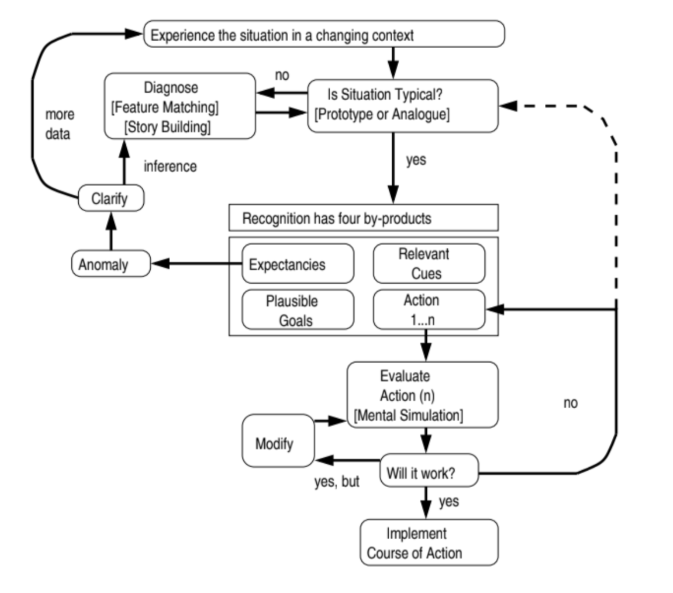
\includegraphics{Figures/klein.PNG}
\decoRule
\caption[ La version intégrée  du modèle de Klein de décision axée sur la reconnaissance] { La version intégrée  du modèle de Klein de décision axée sur la reconnaissance
(Figure 7.1 du livre “Sources of Power” by G. Klein 1998 \parencite{klein2017sources}) }
\label{fig:klein}
\end{figure}


~\par
Ce modèle [Figure \ref{fig:klein}, Page \pageref{fig:klein}] exprime l’idée qu’une personne qui acquiert de l’expertise est plus susceptible 
de reconnaître les subtilités entre les situations et de choisir un plan d’action en conséquence.



~\par

\section{Une brève histoire des jeux dans la recherche sur l'IA}

Les jeux ont une longue histoire dans la recherche sur l'IA, remontant au moins à 1949 lorsque Claude Shannon (peu après avoir développé l'entropie d'informations) s'est intéressé à l'écriture d'un programme informatique pour jouer au jeu d'échecs. Dans son article «Programmer un ordinateur pour jouer aux échecs», Shannon écrit:

~\par
“La machine à échecs est un système idéal pour commencer, car: 

~\par
\begin{enumerate}
\item Le problème est clairement défini à la fois dans les opérations autorisées (les mouvements) et dans le but ultime (le maté); 
\item Il n'est ni si simple d'être trivial ni trop difficile pour une solution satisfaisante; 
\item Les échecs sont généralement considérés comme nécessitant une «réflexion» pour un jeu habile; une solution de ce problème nous obligera soit à admettre la possibilité d'une pensée mécanisée, soit à restreindre davantage notre concept de «pensée»; 
\item La structure discrète des échecs s’intègre parfaitement dans la nature numérique des ordinateurs modernes.”

\end{enumerate}

C'était en 1949.

~\par
Depuis lors, il existe un intérêt durable pour la création de programmes informatiques capables de jouer à des jeux aussi habiles que des joueurs humains, même en battant les champions du monde respectifs. Shannon a inspiré le travail fondateur d’Arthur Samuel sur Checkers dans les années 1950 et 1960. Si le programme de Samuel n’a pas pu battre les experts, il a été considéré comme une réalisation majeure, car il s’agissait du premier programme à utiliser efficacement les procédures de recherche heuristique et les méthodes basées sur l’apprentissage. \parencite{unity1}


~\par
Chinook, un programme de contrôleurs mis au point à l’Université de l’Alberta en 1989, a commencé à battre les joueurs les plus humains et, dès 1994, les meilleurs joueurs pouvaient au mieux égaliser la machine. Cette tendance s’est poursuivie avec d’autres jeux de plateau à 2 joueurs tels que Backgammon (avec TD-Gammon de Gerald Tesauro, 1992-2002) et Chess (lorsque Deep Blue d’IBM a battu Garry Kasparov, 1997), et plus récemment avec Go.

~\par
Une avancée scientifique importante de ces dernières années a été celle où, en 2016, AlphaGo de DeepMind a battu le champion du monde 18 fois Lee Sedol 4 à 1, faisant l’objet du documentaire Netflix, AlphaGo. 



 % Chapter Template

\chapter{BDI ( Belief-Desire-Intention)} % Main chapter title

\label{Chapter4} % Change X to a consecutive number; for referencing this chapter elsewhere, use \ref{ChapterX}

%----------------------------------------------------------------------------------------
%	SECTION 1
%----------------------------------------------------------------------------------------

Les agents du modèle BDI sont basés sur les concepts philosophiques d'intentions, de plans et de raisonnements pratiques développés par Bratman \parencite{bratman1987intention}. Ce modèle est basé sur la psychologie populaire, c'est-à-dire la manière dont nous pensons. Le modèle fournit une première approximation de la cognition humaine, mais il reste encore beaucoup à faire pour l’affiner.


\section{Belief}

Les croyances d'un agent sont sa vision du monde, qui n'est pas nécessairement la même chose que l'état du monde, car les capteurs peuvent être imparfaits, en effet, les informations fournies peuvent être à la fois incomplètes et bruyantes.

\section{Desire}

Plutôt que les désirs d’un agent, nous nous référons à ses objectifs. Ceux-ci donnent l'état du monde dans lequel l'agent souhaite être et doit être cohérent.


\section{Intention}

Ses intentions sont les plans qu'il exécute actuellement. Il peut y avoir plus d'un plan en cours, car un agent peut travailler simultanément à plusieurs objectifs (non conflictuels). Une fois qu'un agent a formulé une intention (c.-à-d. il sélectionne un plan), il est en quelque sorte engagé dans ce plan - il continue de l'exécuter (ou du moins a l'intention de l'exécuter) jusqu'à ce que l'objectif soit atteint ou qu’il devienne impossible à atteindre en suivant ce même plan, l'objectif devient alors inutile. 
Un plan est une «recette» pour atteindre un objectif particulier. C'est une séquence d'actions et/ou de sous-objectifs à réaliser. Si une étape de la séquence échoue, le plan lui-même échouera. L'une des caractéristiques d'un système BDI est que, lorsqu'un plan échoue, l'agent réessaye (si possible). Il tentera de trouver un autre moyen d’atteindre l’objectif en tenant compte du fait que le monde (et donc les convictions de l’agent ou son désir) est en train de changer. Un agent stocke ses plans dans une bibliothèque de plans.


\section{Agent BDI}

L'agent montré à la Figure \ref{fig:bdi}, Page \pageref{fig:bdi} passe par un cycle continu de:

\begin{enumerate}
\item visualiser son environnement;
\item raisonner sur les croyances, les objectifs et les intentions;
\item accomplir une ou plusieurs actions.
\end{enumerate}

Ce cycle est très similaire à celui utilisé dans SWARMM section \ref{ssec:swarm}, qui sépare la deuxième étape en deux étapes: évaluation de la situation suivie de la sélection tactique. En effet, SWARMM est implémenté en utilisant une architecture BDI. Au cours de la phase de raisonnement du cycle, l'agent doit raisonner sur les croyances (si et comment elles devraient changer), les objectifs (les changements de croyances peuvent affecter la faisabilité des objectifs) et les intentions (les changements d'objectifs peuvent amener l'agent à abandonner certaines intentions et / ou d’en créer de nouvelles). L'agent doit également décider quelle action (ou quelles actions) effectuer ensuite, à partir des intentions actuelles.


\begin{figure}[th]
\centering
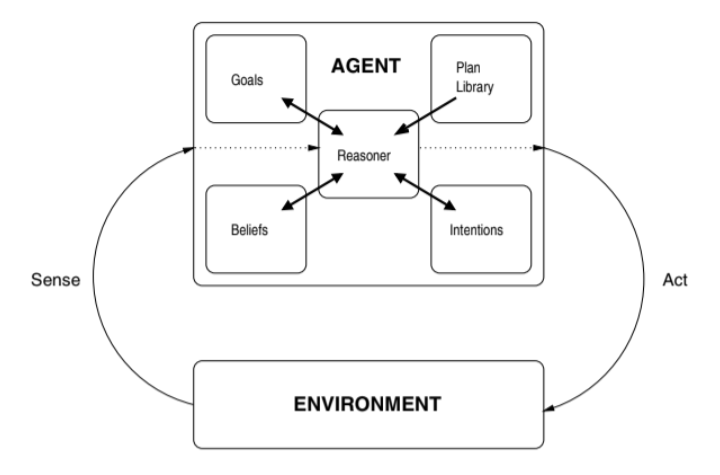
\includegraphics{Figures/bdi.PNG}
\decoRule
\caption[ Structure d’un agent BDI ] { Structure d’un agent BDI }
\label{fig:bdi}
\end{figure}


~\par
Lorsqu'il existe plusieurs plans disponibles pour atteindre un objectif donné, l'agent utilise en théorie un choix rationnel pour sélectionner un plan \parencite{bratman1988plans}. C'est-à-dire que les avantages de tous les plans applicables sont évalués et que le «meilleur» est sélectionné. Cependant la recherche en NDM indique que ce n'est pas ainsi que les agents humains prennent leurs décisions, et c'est sur cela que le travail doit être fait pour  améliorer le modèle BDI .

~\par
Dans les implémentations pratiques d'architectures BDI, telles que JACK \parencite{jack} ou dMARS \parencite{dmars1997formal}, chaque plan est conçu pour gérer un objectif particulier dans un contexte particulier. Dans ces systèmes, le "contexte" est un ensemble de conditions que l'agent doit croire vraies. Cela permet au programmeur de spécifier différentes manières d'atteindre le même objectif dans différentes situations, mais il est également possible d'avoir plusieurs plans applicables dans une situation donnée (lorsque les contextes se chevauchent).
 
% Chapter Template

\chapter{Autres modèles et architectures} % Main chapter title

\label{Chapter5} % Change X to a consecutive number; for referencing this chapter elsewhere, use \ref{ChapterX}

%----------------------------------------------------------------------------------------
%	SECTION 1
%----------------------------------------------------------------------------------------

\section{CogAff}

CogAff est un modèle de traitement de l'information proposé par Sloman \parencite{sloman2005architectural}. Il comprend trois niveaux, à savoir: réactif, délibératif et réflexif (méta-gestion). 
Chaque niveau comprend des mécanismes de perception, des mécanismes de traitement centralisés et des mécanismes d'action. L'architecture possède un mécanisme d'alarme ainsi que des communications d'informations entre toutes les parties de l'architecture. Le mécanisme d'alarme fonctionne de manière centralisée et s'apparente au mécanisme d'interruption.





%-----------------------------------
%	SUBSECTION 1
%-----------------------------------
\subsection{H-CogAff}

H-CogAff est un exemple particulier de CogAff expliquant les phénomènes mentaux humains. Chaque niveau supporte différentes catégories d'émotions. «D'autres subdivisions sont nécessaires pour couvrir toute la variété des émotions humaines, d'autant plus que les émotions peuvent changer de caractère au fil du temps, à mesure qu'elles grandissent» \parencite{sloman2005architectural}.


\section{CLARION}

CLARION a une structure similaire aux trois niveaux de traitement de l’information. C'est une architecture cognitive qui comporte deux niveaux: le niveau implicite (similaire aux niveaux réactifs et de routines) et le niveau explicite (similaire au niveau réflexif). Le niveau implicite est le niveau inférieur et code les connaissances implicites. Il utilise un réseau de neurones multi-couches avec Q-learning pour acquérir des connaissances implicites. Le niveau explicite est le niveau supérieur et code la connaissance explicite. Il utilise un apprentissage ponctuel pour acquérir des connaissances explicites.

~\par
Le niveau le plus bas et le niveau le plus élevé échangent leurs apprentissages au moyen d'un apprentissage ascendant et descendant. Chaque niveau comprend quatre sous-systèmes fonctionnels distincts:

\begin{enumerate}
\item un sous-système centré sur l'action pour contrôler les actions;
\item un sous-système non centré sur l'action pour conserver les connaissances générales implicites ou explicites;
\item un sous-système méta-cognitif pour surveiller, diriger et modifier les opérations de tous les sous-systèmes;
\item un sous-système de motivation pour fournir les motivations sous-jacentes de la perception, de l'action et de la cognition, en termes d'impulsion et de rétroaction.
\end{enumerate}

\section{SHAME}

SHAME (Architecture évolutive et hybride pour le mimétisme des émotions) est un modèle émotionnel ou système simulant l'état émotionnel d'un agent agissant dans un environnement virtuel présenté par Kesteren en 2001 \parencite{kesteren2001supervised}. Il a construit un modèle de simulation à base d'agents appelés «GridWorld». SHAME implémente la fonction d’affect similaire à la fonction d’affect dans le niveau de réflexion et des fonctions de motivation et de comportement similaires à celles du niveau de réactif. Il utilise un réseau de neurones pour apprendre comment l'état émotionnel devrait être influencé par la survenue de stimuli.


\section{Zamin}

Zamin est un environnement de simulation de vie artificielle pour évaluer les capacités des agents à produire un comportement émotionnel et à prendre de meilleures décisions, développé par Zadeh, Shouraki et Halavati \parencite{zadeh2006emotional}. Ces derniers ont mis en place cet environnement afin d’étudier le possible rôle des émotions dans la gestion des ressources mentales. Ils utilisent uniquement un comportement positif/négatif et un comportement d'approche/d'évitement (uniquement la fonctionnalité du niveau réactif) dans un environnement de type prédateur-proie.
 

\chapter{Contribution} % Main chapter title

\label{Chapter6} % Change X to a consecutive number; for referencing this chapter elsewhere, use \ref{ChapterX}

%----------------------------------------------------------------------------------------
%	SECTION 1
%----------------------------------------------------------------------------------------

\section{Unity}

Unity le logiciel que j'utilise pour développer mon framework, c’est est un moteur de jeu multiplateforme (smartphone, ordinateur, consoles de jeux vidéo et Web) développé par Unity Technologies. Il est l'un des plus répandus dans l'industrie du jeu vidéo, aussi bien pour les grands studios que pour les indépendants du fait de sa rapidité aux prototypages et qu'il permet de sortir des jeux sur tous les supports.


~\par
En terme d’intelligence artificielle, ce dernier propose une multitude de fonctionnalités notamment basées sur l’apprentissage (Machine Learning) afin de construire des agents autonomes, conscients de leur environnement et qui interagissent avec selon des paramètres précis, objectifs, actions et réactions.

~\par
L’un des facteurs qui m’ont poussé à l’utiliser et aussi le fait qu'il a la particularité de proposer une licence gratuite dite « Personal » avec quelques limitations de technologie avancée au niveau de l'éditeur, mais sans limitation au niveau du moteur.  



\section{Le Jeu open source “Do not shoot Aliens” - Jeu Mobile}

L'idée principale derrière est de complètement transformer les mécanismes que l’on attend d'un jeu de tir classique, en effet,  au lieu de viser et de tirer afin de vaincre ses ennemis, le personnage du joueur est un peu agressif et décide de tirer sur tout ce qui est autour de lui. 

Le but du joueur est d’atteindre le moins de personnages extraterrestres pour ne pas les contrarier.

Plus les extraterrestres sont touchés, plus le jeu sera difficile, car le joueur devra les frapper une seconde fois pour les arrêter. [Figure \ref{fig:7.2}] 

La victoire est basée sur le fait d’accumuler le plus de points possible en allant de checkpoint en checkpoint.

\begin{figure}[th]
\centering
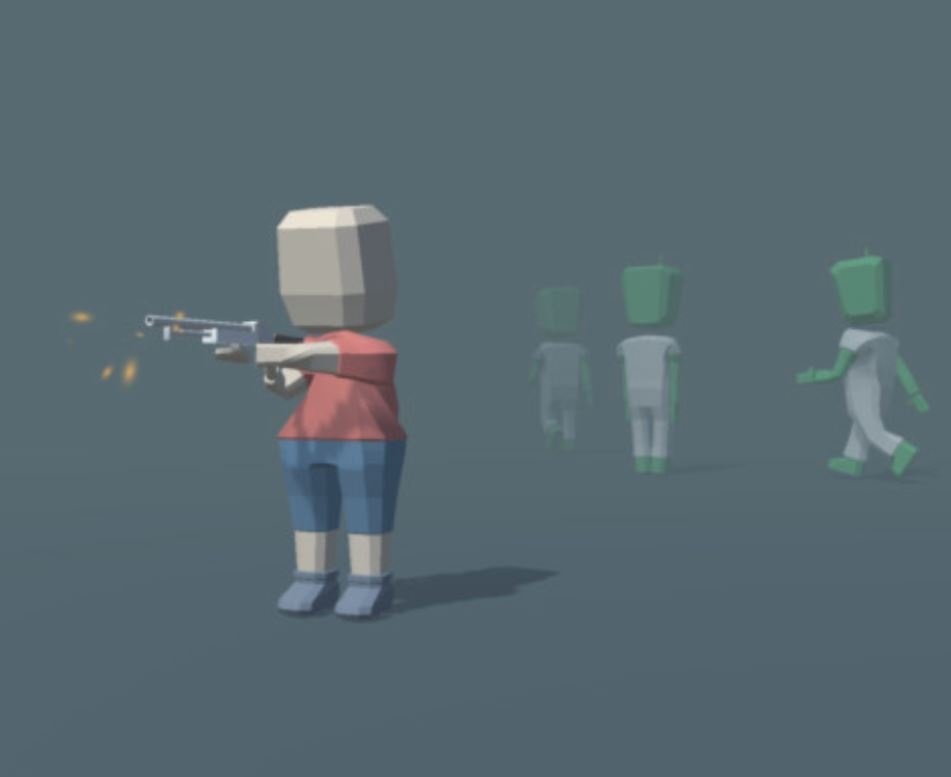
\includegraphics{Figures/72unity.JPG}
\decoRule
\caption[Icon du jeu "Do Not Shoot Aliens"]{Icon du jeu "Do Not Shoot Aliens"}
\label{fig:7.2}
\end{figure}

\section{Langage de programmation}

Chaque agent de ce jeu, que ce soit le personnage principal contrôlé par le joueur ou les agents autonomes représentés ici par les ennemis et même l’environnement ou les objets qui interagissent avec les agents, est géré par un code source qui lui est propre, ce dernier est écrit en C-Sharp, un langage scripté qui permet ensuite au moteur de jeu de le compiler et de l'interpréter, et cela, afin de garantir les meilleures performances de jeu.

~\par
Ce langage est orienté objet, ce qui fait sens car tous les objets, environnements, agents ou encore joueurs sont effectivement des objets 3D, ayant des paramètres qui leur sont propres ( Vitesse, durée de vie, couleur, objectif ) ainsi que de nombreuses fonctions ( marcher, courir, frapper, sauter etc…) qui leur permettent d’effectuer des actions, cette définition nous renvoie au concept de classe, variables de classes et méthodes de classe présentes dans les langages orientés objet.


\section{Description des agents autonomes présents dans le jeu}

Le scénario typique pour la formation d’agents dans des environnements virtuels consiste à avoir un environnement et un agent uniques qui sont étroitement couplés. Les actions de l'agent modifient l'état de l'environnement et lui procurent des récompenses. \parencite{unity2}  

~\par
Dans notre cas, les agents ont pour environnement l’esplanade sur laquelle ils circulent, ils peuvent effectuer des actions par exemple:  marcher doucement, courir ou encore attaquer.
 
 
~\par 
Leur objectif initial est celui de rester “tranquille”, en effet, tant qu’ils ne sont pas touchés, ils conservent leur démarche lente et continuent de circuler de manière hasardeuse (fonction random qui génère leur position dans l’espace).

~\par
Par contre s'ils venaient à être touchés par les balles du joueur principal, leur comportement change et leur objectif aussi, ils se concentrent alors principalement sur l’attaque du personnage principal afin de s’en débarrasser.

On peut identifier ici un exemple de BDI (décrit plus haut): 

\begin{itemize}
\item Leur "Belief" ( ou croyance ) initiale est de croire que leur environnement est inoffensif, c’est leur vision du monde.
\item Ce qui engendre leur désire ou encore leur objectif, qui est de circuler dans l’environnement qui les entoure, ceux-ci décrivent l'état du monde parfait dans lequel ils aimeraient évoluer.
\item Leur "Intention" est ici le plan d’action en cours d'exécution, c’est-à-dire, le fait de déambuler sur l’esplanade.
\end{itemize}


~\par
Comme vu précédemment, tout changement dans leur environnement peut produire un changement dans leur perception de ce dernier, et donc engendrer un nouveau plan d’action, c’est sur ce principe que je me base afin d’appliquer à ces gens différents paramètres qui leur permettront de réagir à leur nouvel environnement. 

\section{Application de paramètres de prises de décisions en milieu naturel (NDM) aux agents BDI}

Afin d’appliquer ces paramètres, je procède de la manière suivante [Figure \ref{fig:75}] : 

\begin{itemize}
\item Je déclare des paramètres qui permettent d’évaluer l’état émotionnel des agents lors des différents changements de l’environnement.
\item Ces variables sont: la peur, la joie, la tristesse et la colère qui sont des booléens.
\item Chaqu’une de ces variable a, à son tour des paramètre qui lui sont étroitement liées: la vitesse de la démarche, ainsi que la couleur des agents.
\item En l'occurrence, la couleur associée à la joie est le jaune.
\item Celle associée à la tristesse est le bleue.
\item Celle associée à la colère est le rouge.
\item Celle associée à la peur est le vert. [Figure \ref{fig:751u}, Page \pageref{fig:751u}]
\end{itemize} 

\begin{figure}[th]
\centering
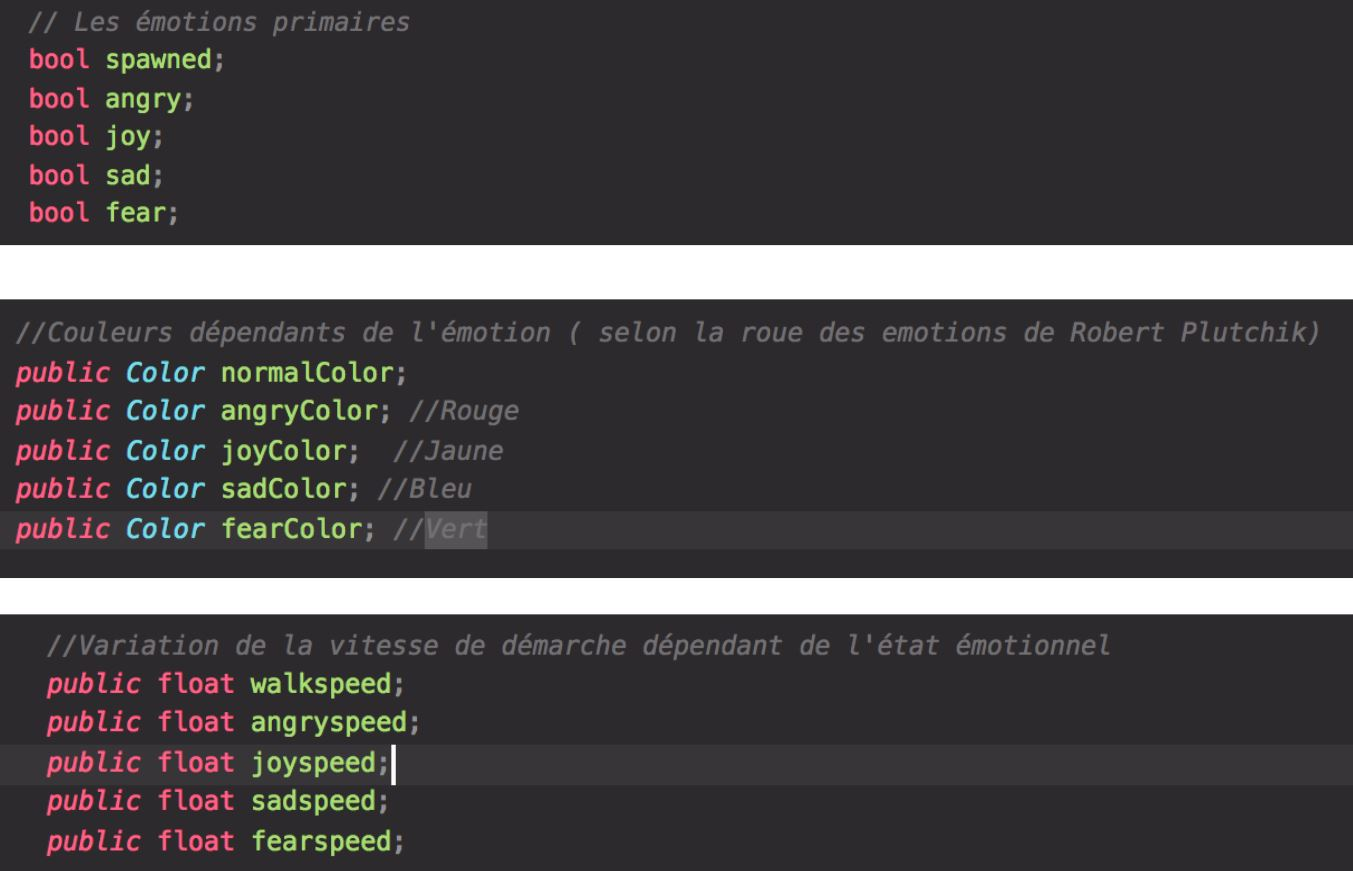
\includegraphics{Figures/75unity.JPG}
\decoRule
\caption[Déclaration des variables]{Déclaration des variables}
\label{fig:75}
\end{figure}



\begin{figure}[th]
\centering
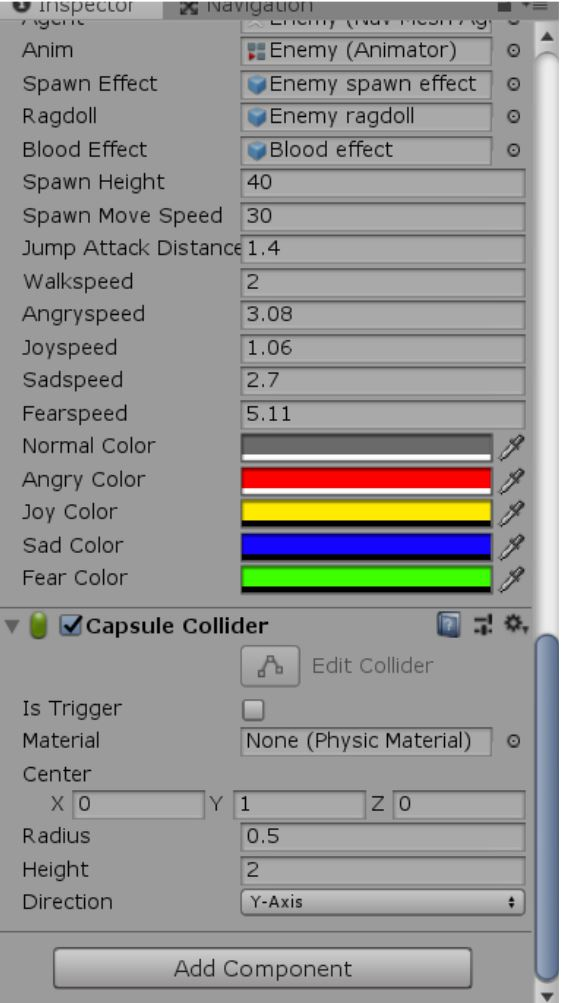
\includegraphics{Figures/751unity.JPG}
\decoRule
\caption[Fenêtre Unity, Valeurs des paramètres]{Fenêtre Unity, Valeurs des paramètres}
\label{fig:751u}
\end{figure}


\subsection{Première expérimentation}

Lors de ma première expérimentation, j’ai décidé d’établir une distance critique entre le joueur et les agents autonomes, lorsque ce dernier est très proche d’eux, qui serait synonyme de tristesse pour ces derniers, sentiment lié au fait de savoir que le jour peut à tout moment les toucher.


\begin{figure}[th]
\centering
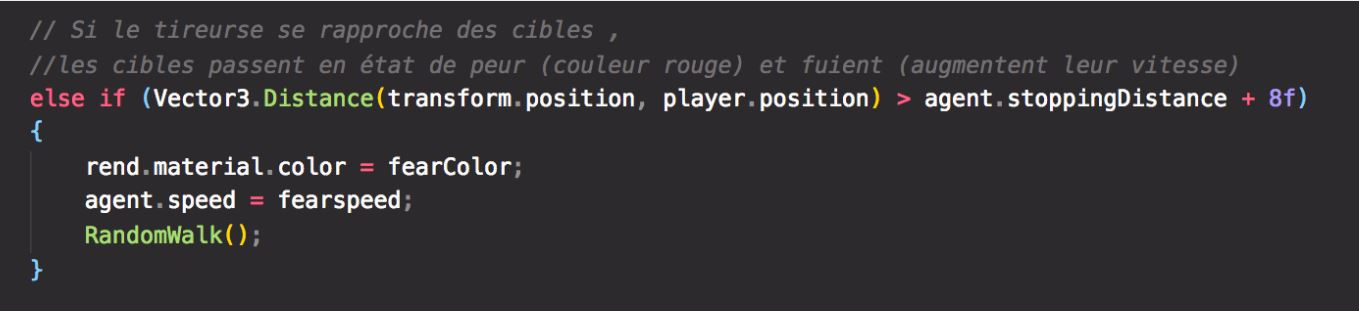
\includegraphics{Figures/fonctdist.JPG}
\decoRule
\caption[Code source implémentant une courte distance ]{Code source implémentant une courte distance entre le jouer et l'agent}
\label{fig:751}
\end{figure}



~\par
La distance est exprimée ici par la position de l’agent en mode “stop” ou à l'arrêt (qui survient lorsque l’agent rencontre sur son chemin ou “path” le joueur) et le joueur lui-même, à laquelle on ajoute un delta en nombre flottant représenté ici par le 8f, il suffit ensuite de varier ce nombre flottant afin d’augmenter ou de diminuer le delta, et de calculer la distance qui sépare les agents autonomes(plus ou moins loin selon le delta) du joueur. 

~\par
Le résultat souhaité est de pouvoir appliquer un changement de couleur aux agents suivant l’émotion qu’ils ressentent, dans la figure \ref{fig:751}, c’est la peur, la couleur de l’agent prend donc la couleur associée à la peur [Figure \ref{fig:bichi1}] une fois que ce dernier est à une distance équivalente à un delta de 8, ce dernier change aussi de vitesse de démarche et adopte un rythme plus élevée lui permettant d'échapper au joueur au fur et à mesure que celui-ci se rapproche.( la vitesse liée à la peur est plus élevé que celle liée à “démarche dite normale comme le montre la figure-fenêtre-unity”).


\begin{figure}[th]
\centering
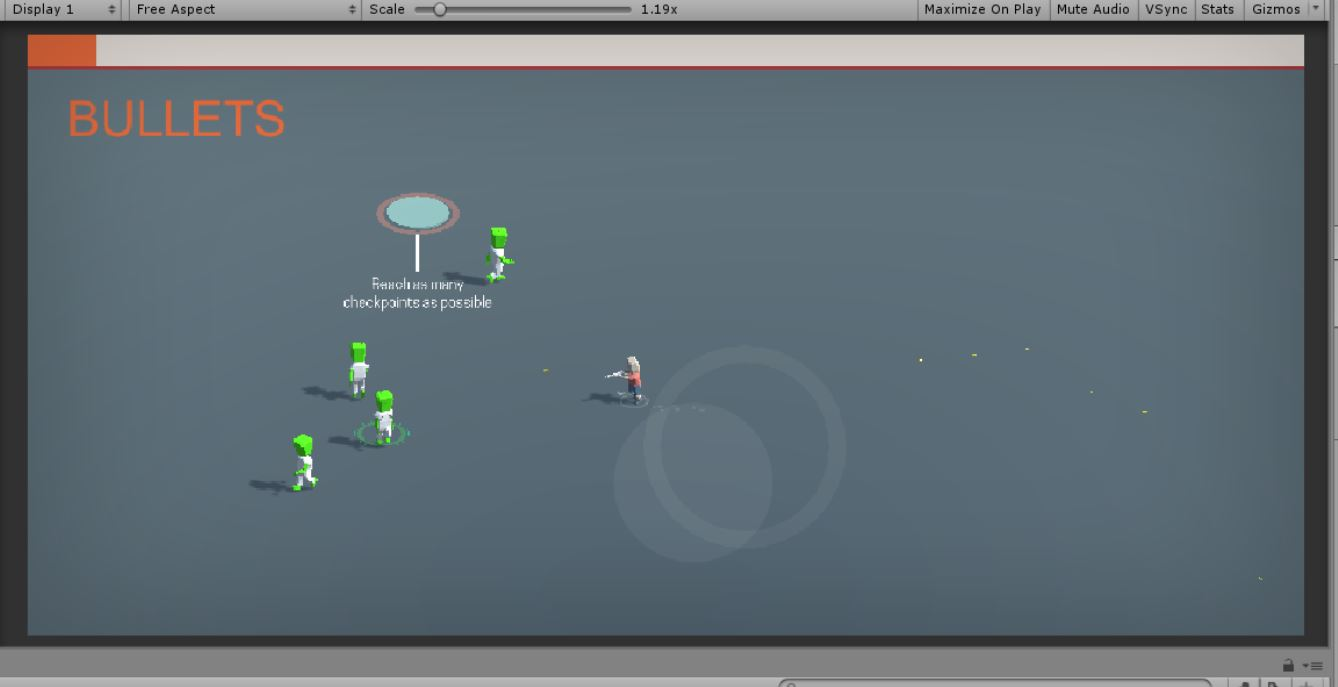
\includegraphics{Figures/bichi1.JPG}
\decoRule
\caption[Visualisation d'agents en état de peur]{Visualisation d'agents en état de peur}
\label{fig:bichi1}
\end{figure}



\subsection{Deuxième expérimentation}

On ajoute cette fois-ci à l'expérience précédente un nouveau facteur émotionnel, celui de la joie.
Suivant le même principe que précédemment, on définit un delta qui permet de calculer la distance entre le joueur et l’agent autonome, celui-ci est de 20f, une distance assez élévée. [Figure \ref{fig:fonct2}]

\begin{figure}[th]
\centering
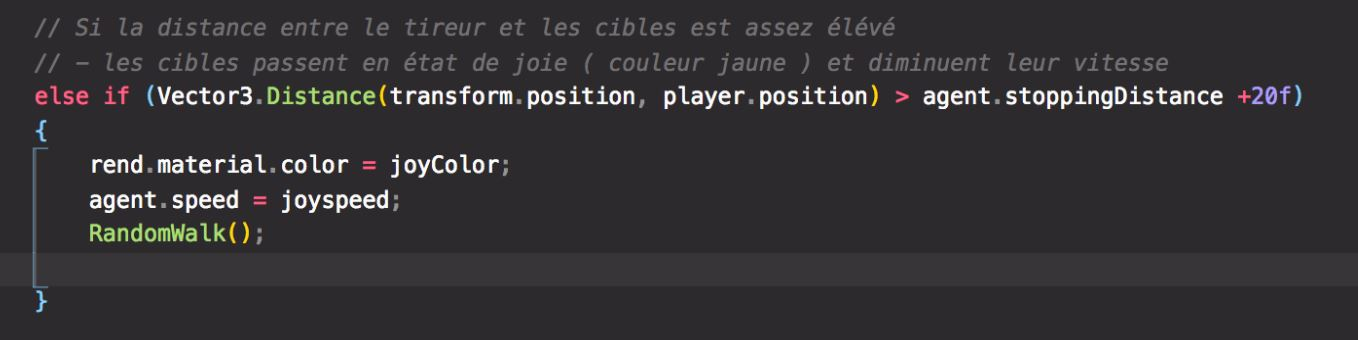
\includegraphics{Figures/fonct2.JPG}
\decoRule
\caption[Code source implémentant une longue distance]{Code source implémentant une longue distance entre le jouer et l'agent}
\label{fig:fonct2}
\end{figure}



~\par
Le résultat souhaité est de pouvoir appliquer un changement de couleur aux agents à l’instant où cette distance entre eux et le joueur est atteints.

~\par
La couleur de ces derniers devient alors jaune, et leur vitesse passe à un rythme beaucoup moins élevée. [Figure \ref{fig:bichi2}]

\begin{figure}[th]
\centering
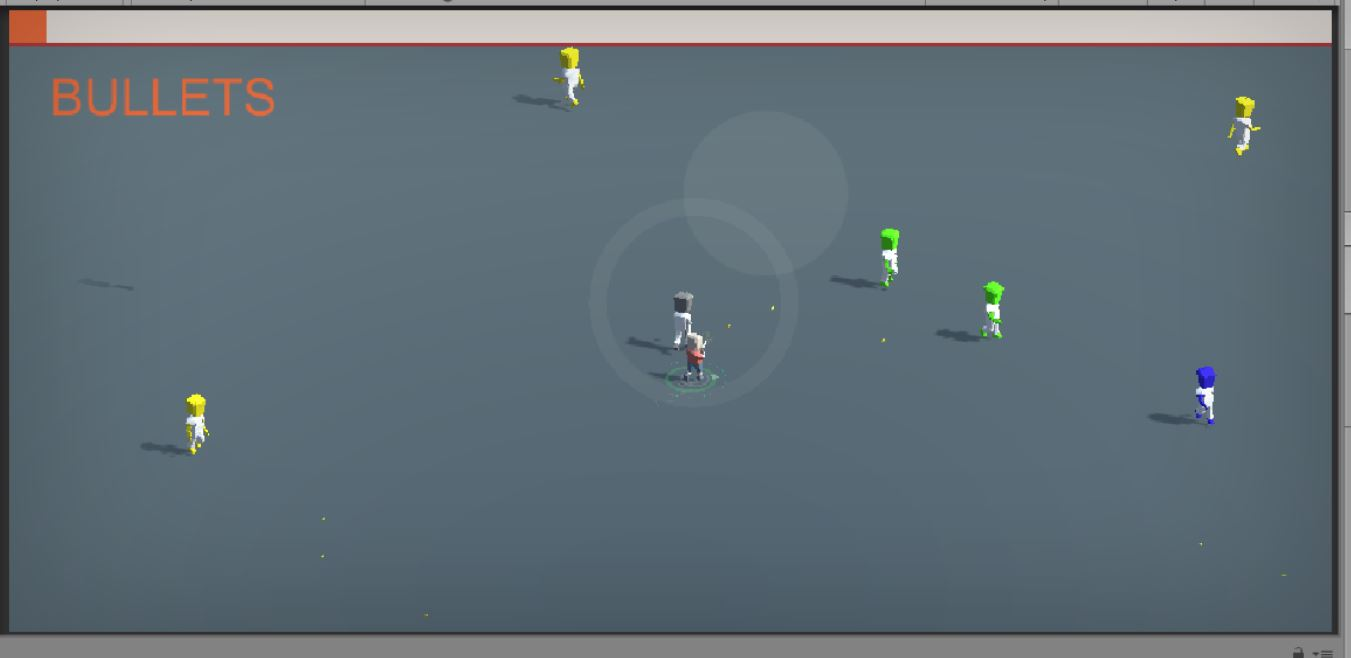
\includegraphics{Figures/bichi2.JPG}
\decoRule
\caption[Visualisation d'agents en état de joie]{Visualisation d'agents en état de joie}
\label{fig:bichi2}
\end{figure}


\subsection{Troisième expérimentation}

On ajoute cette fois-ci à l'expérience précédente un autre facteur émotionnel, celui de la tristesse, ce dernier intervient lorsque la distance équivaut à la valeur médiane entre les deux distances précédentes, c’est-à-dire un delta de 14f. [Figure \ref{fig:333f}]


\begin{figure}[th]
\centering
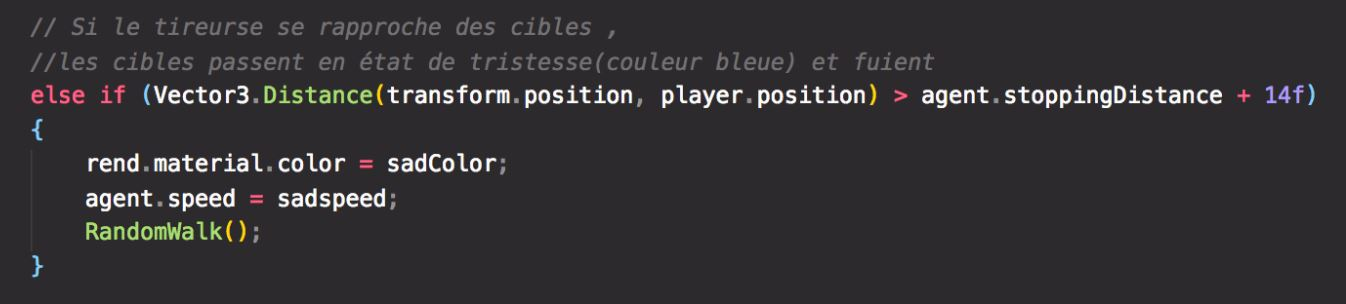
\includegraphics{Figures/333f.JPG}
\decoRule
\caption[Code source implémentant une distance médiane]{Code source implémentant une distance médiane entre le jouer et l'agent}
\label{fig:333f}
\end{figure}

~\par
Le résultat souhaité est de pouvoir appliquer un changement de couleur aux agents à l’instant où cette valeur médiane est atteinte. 


~\par
La couleur de ces derniers devient alors bleue, et leur vitesse passe à un rythme un peu plus soutenu que celui généré par la joie. [Figure \ref{fig:bichi3}]

\begin{figure}[th]
\centering
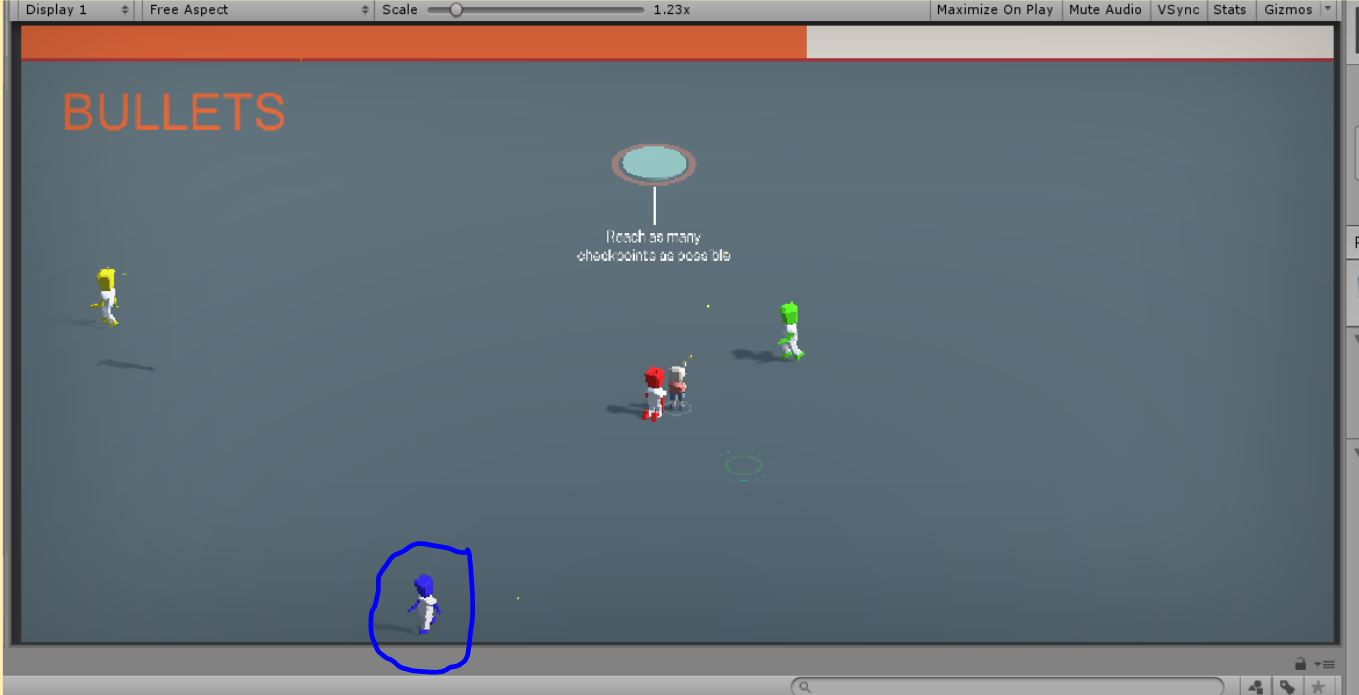
\includegraphics{Figures/bleu.JPG}
\decoRule
\caption[Visualisation d'agents en état de tristesse]{Visualisation d'agents en état de tristesse}
\label{fig:bichi3}
\end{figure}


~\par
Ajoutons à tout cela, le comportement présent dans le code source du jeu [Figure \ref{fig:derfon}], à savoir la colère, celle-ci génère une vitesse plus élevée que toutes les autres chez l’agent autonome, et une couleur noire(définie par moi), en plus de cela, elle change le centre d'intérêt du joueur en terme de démarche, jusque-là ce dernier se déplaçait de manière hasardeuse grâce à la fonction RandomWalk(), une fois le sentiment de colère déclenché, son point d’arrivée se rattache à la position du joueur(comme le montre la figure \ref{fig:bichi4} sur la page \pageref{fig:bichi4}).



\begin{figure}[th]
\centering
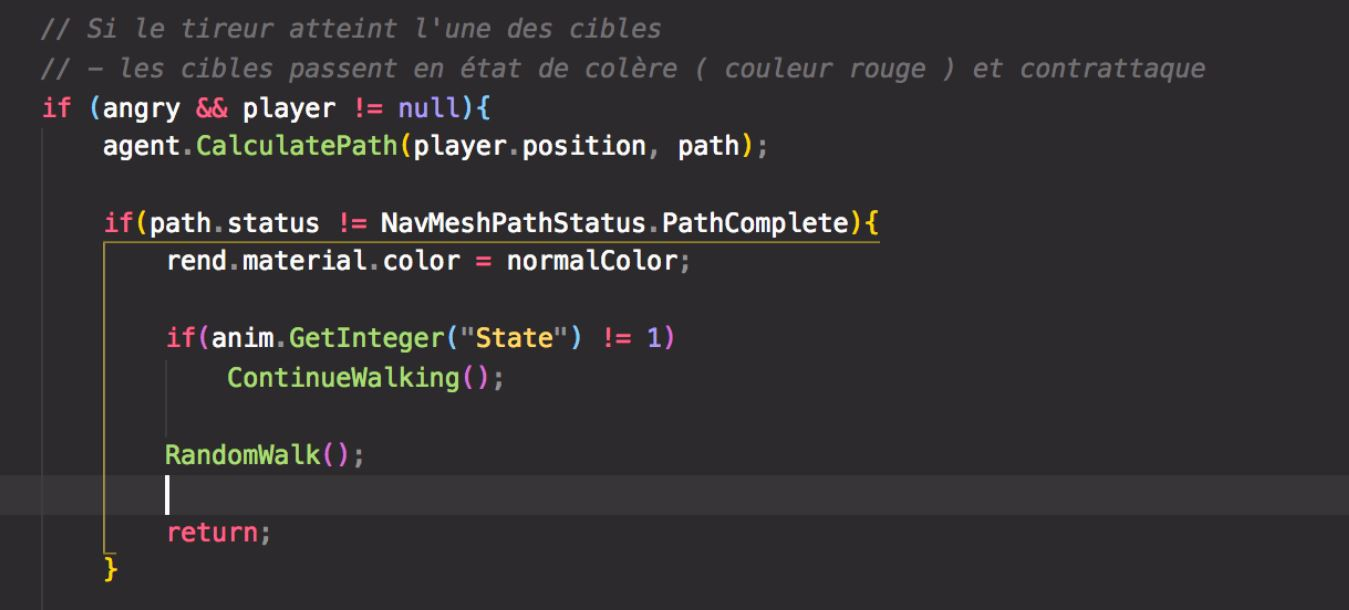
\includegraphics{Figures/derfon.JPG}
\decoRule
\caption[Code source implémentant la réaction d'un agent en état de colère]{Code source implémentant la réaction d'un agent en état de colère}
\label{fig:derfon}
\end{figure}



\begin{figure}[th]
\centering
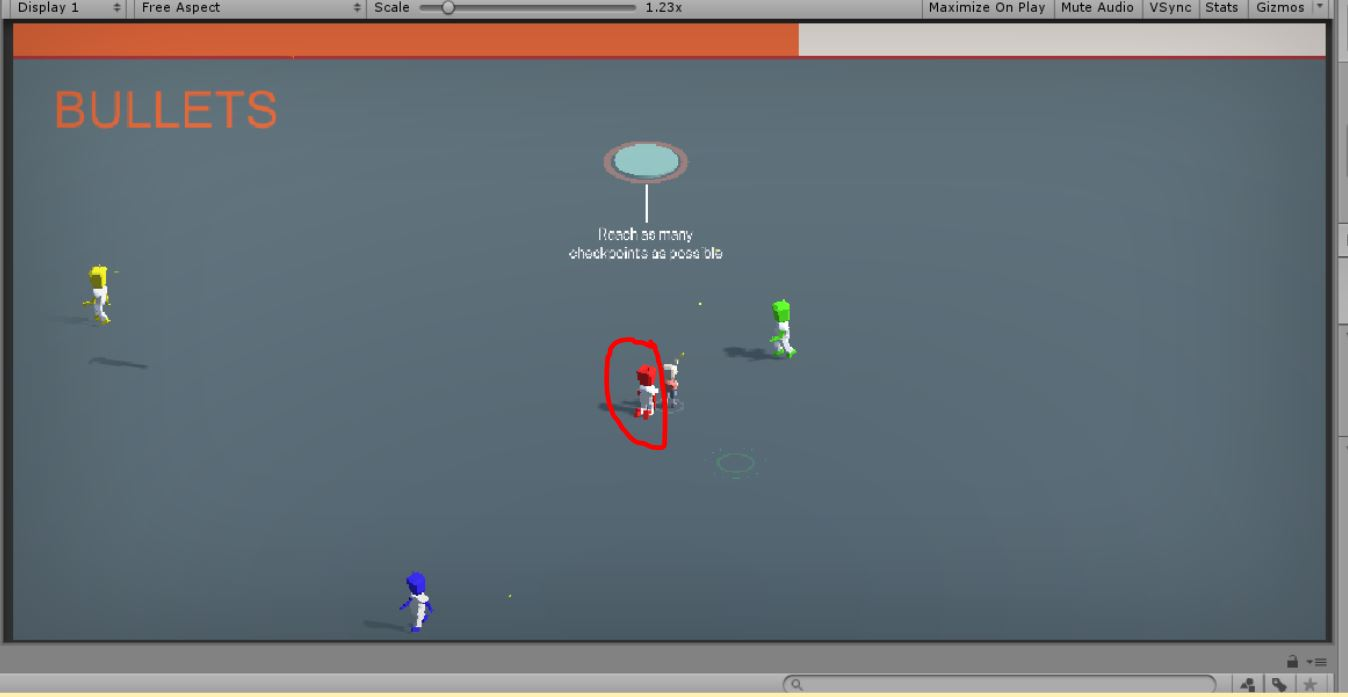
\includegraphics{Figures/rouge.JPG}
\decoRule
\caption[Visualisation d'agents en état de colère]{Visualisation d'agents en état de colère}
\label{fig:bichi4}
\end{figure}

\section{Résultat général (positif/négatifs)}

\subsection{Résultats positifs}

Les résultats suites à ces tests sont plutôt concluants, et confirment l’hypothèse mise en place par le modèle BDI.


~\par
À chaque changement de l’état du monde, rapprochement ou éloignement de l’agent représentant la menace, les paramètres considérées, de joie, de peur, de tristesse ou de colère changent et influent sur la réaction des agents et leur comportement.


~\par
Le passage entre différentes émotions fonctionne quant à lui aussi très bien, par exemple, si le joueur se rapproche beaucoup des agents, ceux-ci prennent peur et changent leurs démarches afin d’aller plus vite et de fuir, mais si l’agent s’éloigne d’eux, les agents reprennent petit à petit une démarche normale (jusqu’à ce que la distance les séparant soit assez élevé pour qu’ils puissent considérer qu’il n’y a plus de danger), ainsi qu’une couleur correspondant à leur nouvelle émotion.


~\par
On peut remarque les prises de décisions sont donc peu “rationnels”, et plus “naturels”, même si quelques points négatifs restent observables.

\subsection{Résultats négatifs}

L’un des points négatifs peut se résumer dans le passage d’une émotion à une autre qui n’est pas à mon sens pas assez réaliste, en effet dans la réalité, un agent humain peut mettre plusieurs minutes, plusieurs heures voient plusieurs jours ou mois pour se passer d’une émotion à une autre, ou se débarrasser d’une émotion désagréable liée à des situations particulières telles que des traumatismes.

~\par
Pouvoir appliquer cela dans un jeu vidéo, implique d'après moi d’ajouter des facteurs temporels à chaque émotion, facteur temporel d'acquisition de l’émotion et facteur temporel de disparition(dismiss) de l’émotion, ainsi que des facteurs d’intensité, en effet, les études sur les êtres humains montrent que toutes les émotions ne se valent pas en terme d’intensité, de manifestation physique ou psychologique.







 
\chapter{Conclusion} % Main chapter title

\label{Chapter7} % Change X to a consecutive number; for referencing this chapter elsewhere, use \ref{ChapterX}

Pour conclure, nous pouvons constater à partir des recherches faites sur les SMA (systèmes multi-agents) ainsi que leurs domaines d’application suivant  différents modèles de programmation telle que le modèle BDI (Belief, Desire, Intention) (Exemple du “SWARMM”) que la plupart des agents autonomes  actuellement en opération procèdent de manière très rationnelle dans leur prise de décision.

~\par
Cela se fait suite à une sélection de multiples possibilités, et élection de celle ayant le plus haut “score” qui est aussi celle-ci ayant prouvé son fonctionnement dans les situations précédentes équivalentes à celle en cours d'exécution.

~\par
Ainsi, différents chercheurs se sont penchés sur la question afin de rendre ces agents plus réalistes et crédible aux yeux de l’homme, leurs recherches, d’abord sur l’homme ont prouvé que ce dernier n'effectue un choix rationnel dans une situation donnée au sein d’un environnement donné que très rarement, ils ont en conclue différents modèles dit “Naturels” ou NDM “prise de décisions en milieu naturel” basés sur le comportement des agents humains, notamment ceux qui sont les plus compétents dans le domaine étudié, de manière individuelle ou en groupes, dans un environnement dynamique, rapide et incertain.

~\par
Le but était donc ensuite de pouvoir appliquer ces mêmes schémas de pensées et de sélections à des agents autonomes, de nombreux modèles ont en effet vu le jour suite à ces recherches, principalement destinés à l’aide à la décision, ou pour développer de meilleurs modèles cognitifs pour les humains lors des simulations.

~\par
Ma contribution dans ce domaine a montré qu’il était possible d’établir certaines règles simples dans un environnement donné constitué d’agents autonomes, qui permettent de simuler des émotions, basées sur des facteurs physiques, de distance, temporels ou encore de prédation, ces règles peuvent influer sur le comportement de ces agents de manière concrète, c’est-à-dire engendrer des actions suite à des changements dans leur environnement, changements qui influent sur leur état ou émotion du moment et les poussent à repenser leur monde où en tout cas, la vision qu’ils s’en font, et donc de penser un nouveau plan d’action selon l’évolution de leurs émotions.

~\par
L’exemple que j’ai pris peut-être très facilement amélioré en intégrant des données plus détaillées sur les émotions comme les  facteurs de temps, qui peuvent être issuent de la psychologie humaine, ou encore les facteurs d'intensités, qui peuvent être déduites d'expériences issuent de situations réelles. ce qui rendrait le passage d’une émotion à une autre plus réaliste et donc plus crédible à l’oeil de l’homme.
 

%----------------------------------------------------------------------------------------
%	THESIS CONTENT - APPENDICES
%----------------------------------------------------------------------------------------

\appendix % Cue to tell LaTeX that the following "chapters" are Appendices

% Include the appendices of the thesis as separate files from the Appendices folder
% Uncomment the lines as you write the Appendices

% Appendix A

\chapter{Code source de personnages non jouables du jeu "Do Not Shoot Aliens"} % Main appendix title

\label{AppendixA} % For referencing this appendix elsewhere, use \ref{AppendixA}


\begin{lstlisting}[language=Csh]

using System.Collections;
using System.Collections.Generic;
using UnityEngine;
using UnityEngine.AI;

public class Enemy : MonoBehaviour {
    
	public NavMeshAgent agent;
	public Animator anim;
	public GameObject spawnEffect;
	public GameObject ragdoll;
	public GameObject bloodEffect;
	
	public float spawnHeight;
	public float spawnMoveSpeed;
	public float jumpAttackDistance;

    #Variables de la vitesse dépendantes de l'état de l'émotion
    public float walkspeed;
    public float angryspeed;
    public float joyspeed;
    public float sadspeed;
    public float fearspeed;

    #Couleurs dépendantes de l'émotion ( selon la roue des émotions de Robert Plutchik)
    public Color normalColor;
    public Color angryColor; #Rouge
    public Color joyColor;  #Jaune
    public Color sadColor; #Bleu
    public Color fearColor; #Vert

    Transform player;
	MoveArea area;
	GameManager manager;

    #Les émotions primaires 
    bool spawned;
    bool angry;
    bool joy;
    bool sad;
    bool fear;

    Vector3 randomTarget;
	NavMeshPath path;
	Renderer rend;
	
	void Start(){
		PlayerController controller = GameObject.FindObjectOfType<PlayerController>();
		
		if(controller != null)
			player = controller.gameObject.transform;
		
		area = GameObject.FindObjectOfType<MoveArea>();
		manager = GameObject.FindObjectOfType<GameManager>();
		
		rend = GetComponentInChildren<Renderer>();
		rend.material.color = normalColor;
		
		path = new NavMeshPath();
	
		agent.speed = walkspeed;
		agent.enabled = false;
		
		Instantiate(spawnEffect, transform.position, transform.rotation);
		transform.Translate(Vector3.up * spawnHeight);
	}
	
	void Update(){
		if(!spawned){
			transform.Translate(Vector3.up * Time.deltaTime * -spawnMoveSpeed);
			
			if(transform.position.y <= 0){
				transform.position = new Vector3(transform.position.x, 0, transform.position.z);
				spawned = true;
				agent.enabled = true;
				
				anim.SetInteger("State", 1);
				randomTarget = area.RandomPosition();
			}
			
			return;
		}

        # Si le tireur atteint l'une des cibles,
        #les cibles passent en état de colère ( couleur rouge ) et contrattaquent  
        if (angry && player != null){
			agent.CalculatePath(player.position, path);
			
			if(path.status != NavMeshPathStatus.PathComplete){	
				rend.material.color = normalColor;
				
				if(anim.GetInteger("State") != 1)
					ContinueWalking();
				
				RandomWalk();
				
				return;
			}

            rend.material.color = angryColor;
            agent.destination = player.position;
			
			if(anim.GetInteger("State") != 2){
				anim.SetInteger("State", 2);
                agent.speed = angryspeed;
                agent.stoppingDistance = jumpAttackDistance;
			}
			
			if(Vector3.Distance(transform.position, player.position) < agent.stoppingDistance + 0.1f){
				agent.isStopped = true;
				transform.LookAt(player.position);
				anim.SetInteger("State", 3);
				spawned = false;
				
				StartCoroutine(Attack());
			}


         
        }

        # Si la distance entre le tireur et les cibles est assez  
        #élevée, les cibles passent en état de joie ( couleur jaune ) et diminuent leur vitesse
        else if (Vector3.Distance(transform.position, player.position) > agent.stoppingDistance +20f)
        {
            rend.material.color = joyColor;
            agent.speed = joyspeed;
            RandomWalk();

        }

        # Si le tireur se rapproche des cibles ,
        #les cibles passent en état de tristesse(couleur bleue) et fuient 
        else if (Vector3.Distance(transform.position, player.position) > agent.stoppingDistance + 14f)
        {
            rend.material.color = sadColor;
            agent.speed = sadspeed;
            RandomWalk();
        }

        # Si le tireur se rapproche des cibles ,
        #les cibles passent en état de peur (couleur rouge) et fuient (augmentent leur vitesse)
        else if (Vector3.Distance(transform.position, player.position) > agent.stoppingDistance + 8f)
        {
            rend.material.color = fearColor;
            agent.speed = fearspeed;
            RandomWalk();
        }

    


        else
        {
            ContinueWalking();
		}
	}
	
	void ContinueWalking(){
		anim.SetInteger("State", 1);
		randomTarget = area.RandomPosition();
		agent.speed = walkspeed;
		agent.isStopped = false;
		spawned = true;
	}
	
	void RandomWalk(){
		if(Vector3.Distance(transform.position, randomTarget) < agent.stoppingDistance + 0.1f){
			randomTarget = area.RandomPosition();
		}
		else{
			agent.destination = randomTarget;
		}
	}
	
	public void Hit(){
		Instantiate(bloodEffect, transform.position + Vector3.up * 1.5f, transform.rotation);
        if (angry){
			Die();
            # Si l'une des cibles est éliminée, les autres passent en état de tristesse
        }
		else{
			angry = true;
		}
	}
	
	void Die(){
		GameObject newRagdoll = Instantiate(ragdoll, transform.position, transform.rotation);
		newRagdoll.GetComponentInChildren<Renderer>().material.color = angryColor;
       
        Destroy(gameObject);
       
    }
	
	IEnumerator Attack(){
		yield return new WaitForSeconds(0.5f);
		
		if(player != null && Vector3.Distance(transform.position, player.position) > agent.stoppingDistance + 0.1f){
			agent.isStopped = false;
			anim.SetInteger("State", 2);
			spawned = true;
		}
		else{
			manager.GameOver();
			ContinueWalking();
		}
	}
}



\end{lstlisting}

%\include{Appendices/AppendixB}
%\include{Appendices/AppendixC}

%----------------------------------------------------------------------------------------
%	BIBLIOGRAPHY
%----------------------------------------------------------------------------------------

\printbibliography[heading=bibintoc]
%\bibliography{biblio}

%----------------------------------------------------------------------------------------

\end{document}  
